\chapter{Desenvolvimento}
  \section{Requisitos}
	Para cada frente do projeto foram definidos os seguintes requisitos.
	\subsection{Frente de Software}
	\begin{itemize}
		\item Conexão com o servidor do google.
		\item Mostrar as rotas percorridas pela bicicleta.
		\item Definir rotas de acordo com o solicitado pelo usuário.
		\item Enviar informações de rotas para o controlador na bicicleta.
		\item Mostrar dados de distância percorrida.
		\item Mostrar dados de tempo gasto de uma rota percorrida.
		\item Salvar dados no servidor.
		\item Gerar gráfico estatístico do usuário.
	\end{itemize}
 
  \section{Software}
  O escopo do projeto de software busca determinar as fronteiras do projeto em quesitos de processamento e interface, e sua interação direta e indireta com o usuário e com a parte eletroeletrônica do projeto.

Esta seção abordará desde nível mais alto do projeto, contemplando as especificações do aplicativo, ao nível mais baixo, contemplando a comunicação entre o aplicativo e o micro controlador.

	\subsection{Aplicativo}
O projeto de processamento e interface consistirá num aplicativo cujo objetivo central é traçar rotas entre os pontos escolhidos pelo usuário e passar essas informações ao micro controlador responsável por acender os painéis luminosos. 
Em segundo plano estará o painel do usuário, onde ele poderá se cadastrar e acompanhar suas rotas, assim como algumas estatísticas sobre seus percursos.

A partir desses objetivos principais, foi criado as features para o projeto. O diagrama a seguir contempla o diagrama de features do sistema:

%\graphicspath{{figuras/}}
\begin{figure}[!htb]
	\centering
	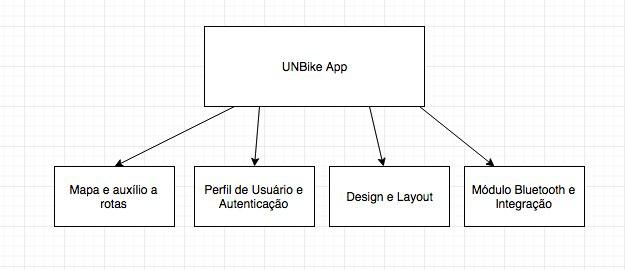
\includegraphics[scale=0.80]{features.jpg}
	\caption{Diagrama de Features}
	\label{img:features}
\end{figure}

Assim foi criado o Product Backlog contemplando uma lista de funcionalidades que são as histórias de usuário que estão vinculadas às features. Artefato importantíssimo que proporciona uma visão macro do projeto. Para melhor visualização, os itens foram divididos em três listas distintas:

A primeira lista, que pode ser vista na figura \ref{img:figura1} contempla os itens críticos ou de alta prioridade.

\graphicspath{{figuras/}}
\begin{figure}[!htb]
\centering
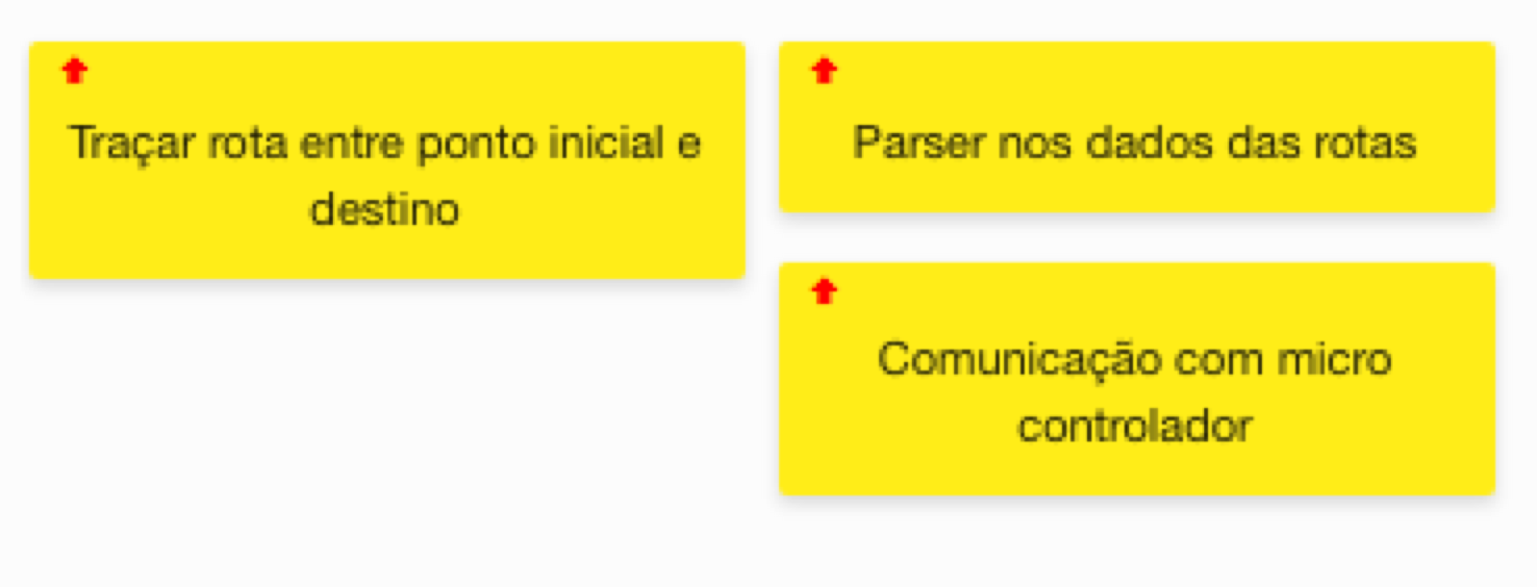
\includegraphics[scale=0.80]{figura1}
\caption{\textit{Backlog} 1}
\label{img:figura1}
\end{figure}

A segunda lista pode ser vista na figura \ref{img:figura2} e evidencia os itens de prioridade normal.

\newpage

\graphicspath{{figuras/}}
\begin{figure}[!htb]
\centering
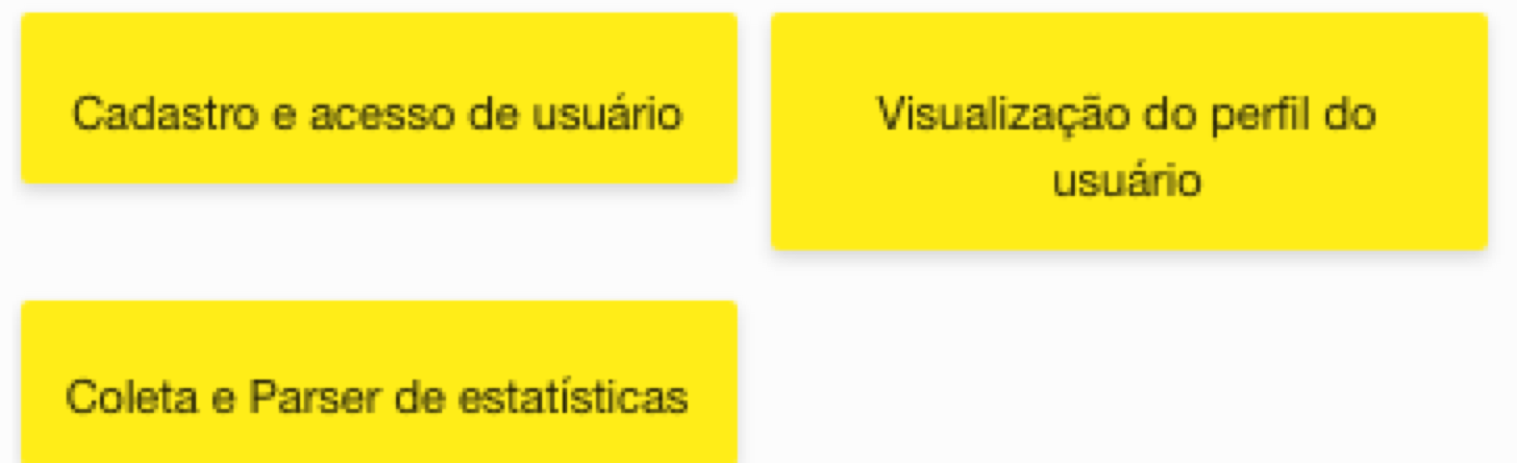
\includegraphics[scale=0.80]{figura2}
\caption{\textit{Backlog} 2}
\label{img:figura2}
\end{figure}

Por fim, a terceira lista mostrada na figura \ref{img:figura3} trata os itens de menor relevância ou de prioridade baixa.

\graphicspath{{figuras/}}
\begin{figure}[!htb]
\centering
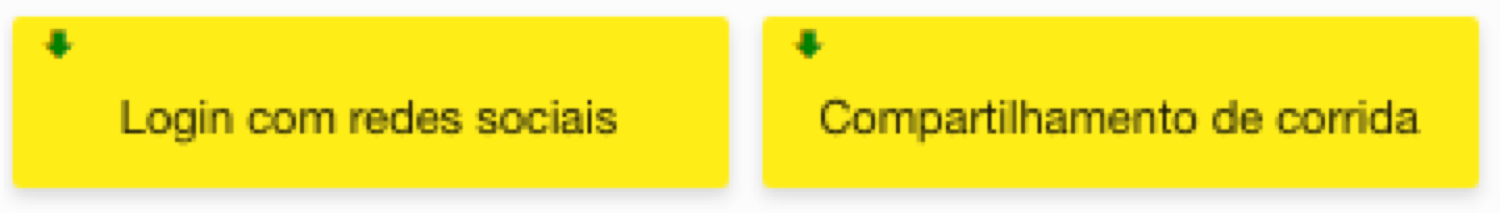
\includegraphics[scale=0.80]{figura3}
\caption{\textit{Backlog} 3}
\label{img:figura3}
\end{figure}

\subsubsection{Solução Técnica}
Nesta seção serão apresentadas as evoluções da subárea de software no decorrer do projeto até a presente data.

O sistema em desenvolvimento compõe:
\begin{itemize}
	\item Aplicação mobile desenvolvida utilizando o framework de desenvolvimento 
	nativo do facebook, React Native;
	\item Servidor de aplicação utilizando Node.JS, servidor que executa o V8 JavaScript,
	interpretador de JavaScript desenvolvido e utilizado pelo google. 
\end{itemize}

O ambiente de desenvolvimento compõe:
\begin{itemize}
	\item Sistema operacional OSX Sierra 10.12.4
	\item Node Versão 5.8.0
	\item React Versão 15.4.0
\end{itemize}

As features implementadas até o ponto de controle 2 foram o mapa e orientação de rotas, o perfil de usuário e autenticação e design e layout.

Pode-se observar que a feature de integração do módulo bluetooth será implementada para o ponto de controle 3, assim como a realização de melhorias no layout e design.

As figuras a seguir mostram algumas telas da execução do aplicativo atualmente:

%\graphicspath{{figuras/}}
\begin{figure}[!htb]
	\centering
	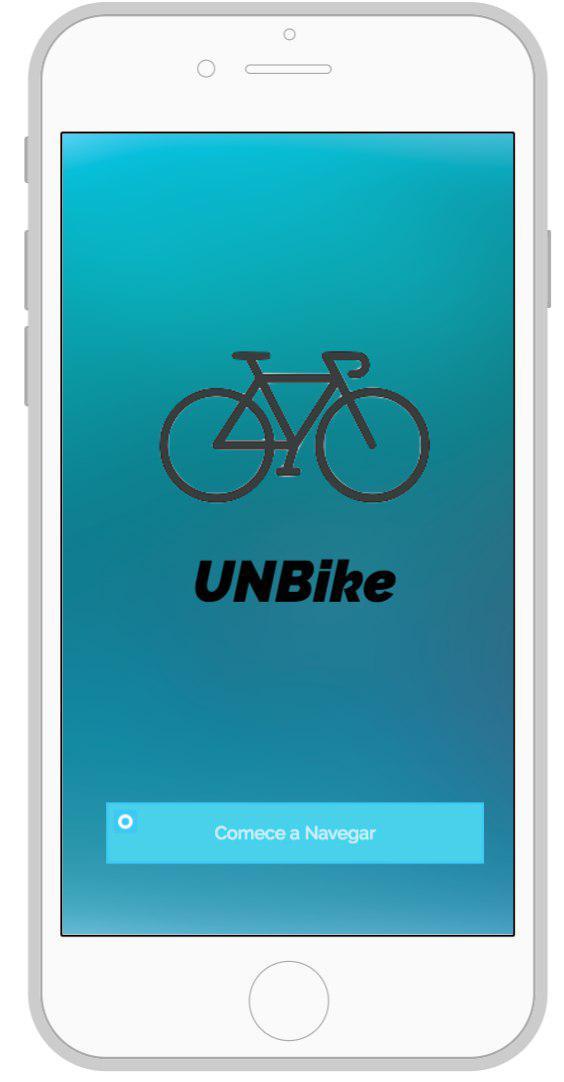
\includegraphics[scale=0.50]{tela_inicial.jpg}
	\caption{Tela Inicial}
	\label{img:telainicial}
\end{figure}

\newpage

\begin{figure}[!htb]
	\centering
	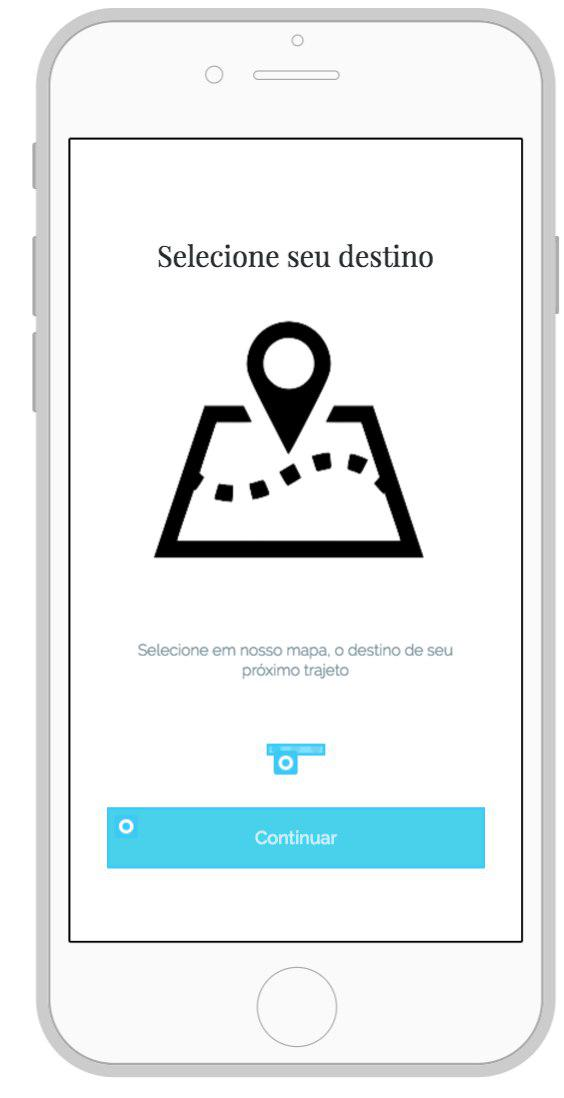
\includegraphics[scale=0.50]{tela_introducao.jpg}
	\caption{Tela de Introdução}
	\label{img:telaintroducao}
\end{figure}

\begin{figure}[!htb]
	\centering
	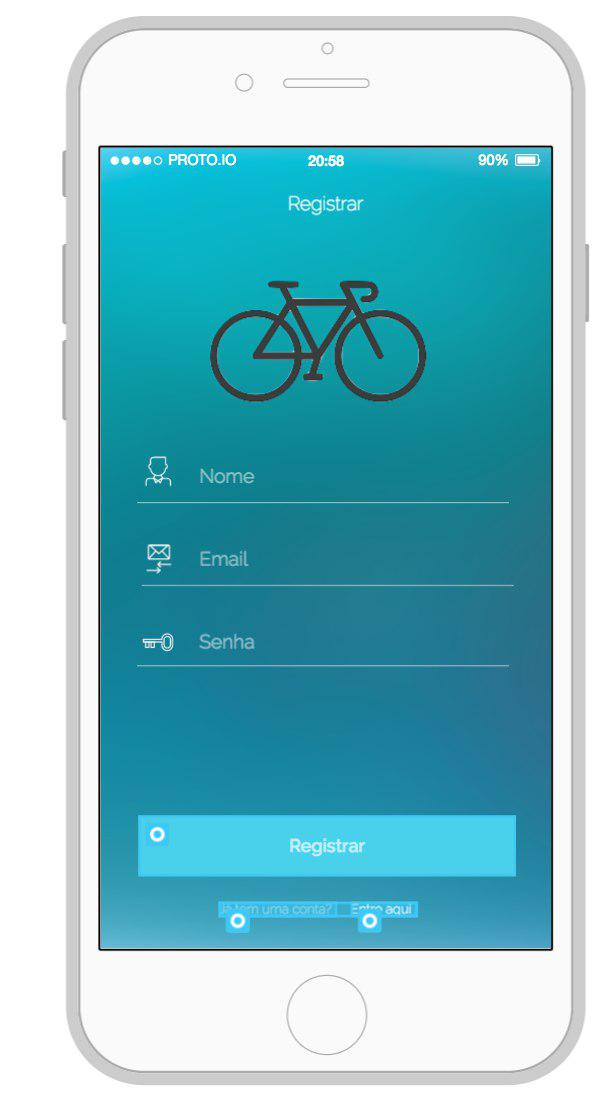
\includegraphics[scale=0.50]{tela_cadastro.jpg}
	\caption{Tela de Cadastro}
	\label{img:telacadastro}
\end{figure}

\begin{figure}[!htb]
	\centering
	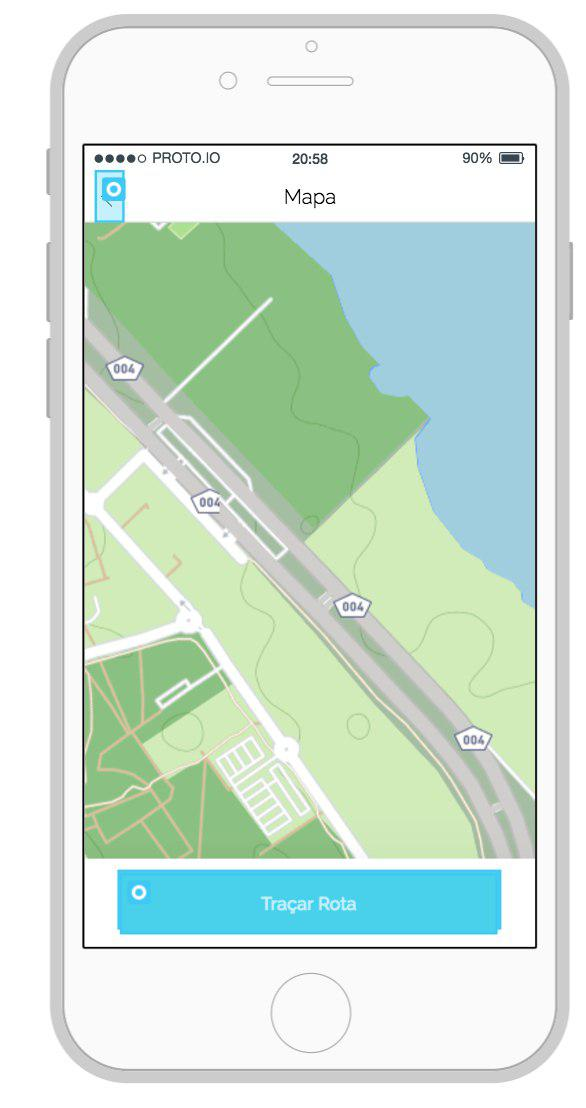
\includegraphics[scale=0.50]{tela_mapa.jpg}
	\caption{Tela de Mapa}
	\label{img:telamapa}
\end{figure}

\begin{figure}[!htb]
	\centering
	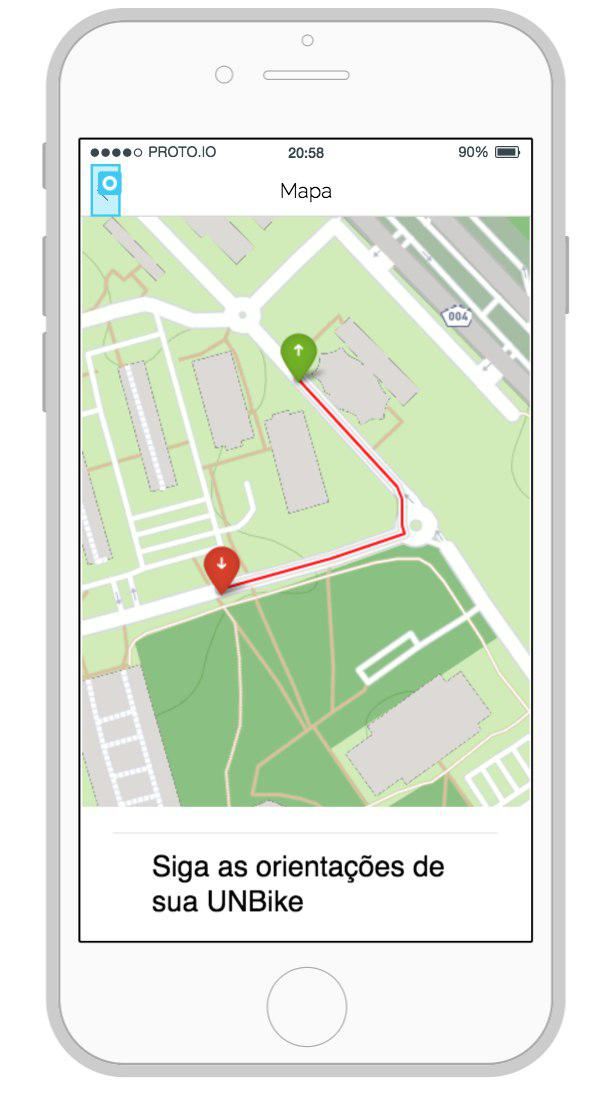
\includegraphics[scale=0.50]{tela_orientacao.jpg}
	\caption{Tela de Orientação}
	\label{img:telaorientacao}
\end{figure}

\begin{figure}[!htb]
	\centering
	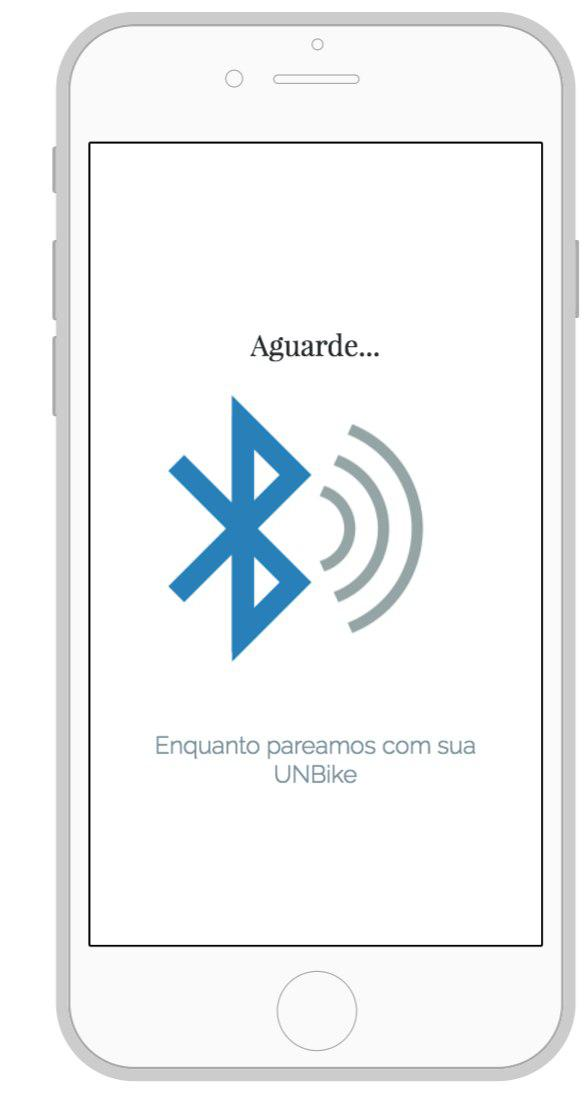
\includegraphics[scale=0.50]{tela_pareamento.jpg}
	\caption{Tela de Pareamento}
	\label{img:telapareamento}
\end{figure}

	\subsection{Arquitetura}
	Aplicativos híbridos são aplicativos feitos utilizando tecnologias web, que depois são convertidos em um aplicativo instalável para celulares e smartphones. Esse tipo de aplicativo funciona como qualquer outro aplicativo e é publicado na loja normalmente.

O React-Native é um projeto desenvolvido pelos engenheiros do Facebook  que consiste em uma série de ferramentas que tornam possível a criação de aplicações Android e iOS. Alguns fatores foram levados em conta para a decisão de se desenvolver um aplicativo híbrido utilizando React-Native neste projeto:

\begin{itemize}
\item Possibilidade de desenvolver aplicativos Android e iOS com apenas uma base de código;
\item Possibilidade de utilizar componentes nativos de cada sistema operacional, desta forma podendo manter a aparência e experiência do aplicativo, consistentes;
\item Compatibilidade com diversas bibliotecas de terceiros,  por exemplo a react-native-ble  com a qual é possível implementar conexões bluetooth;
\item Baixo uso de memória;
\item Conhecimento prévio da equipe de desenvolvimento;
\item Forte comunidade já formada.

\end{itemize}

	Para a comunicação externa, ou seja, para o processamento, será utilizada arquitetura em serviços RESTful.
O design de uma arquitetura REST, segue o padrão evidenciado na figura \ref{img:arquitetura}

\graphicspath{{figuras/}}
\begin{figure}[!htb]
\centering
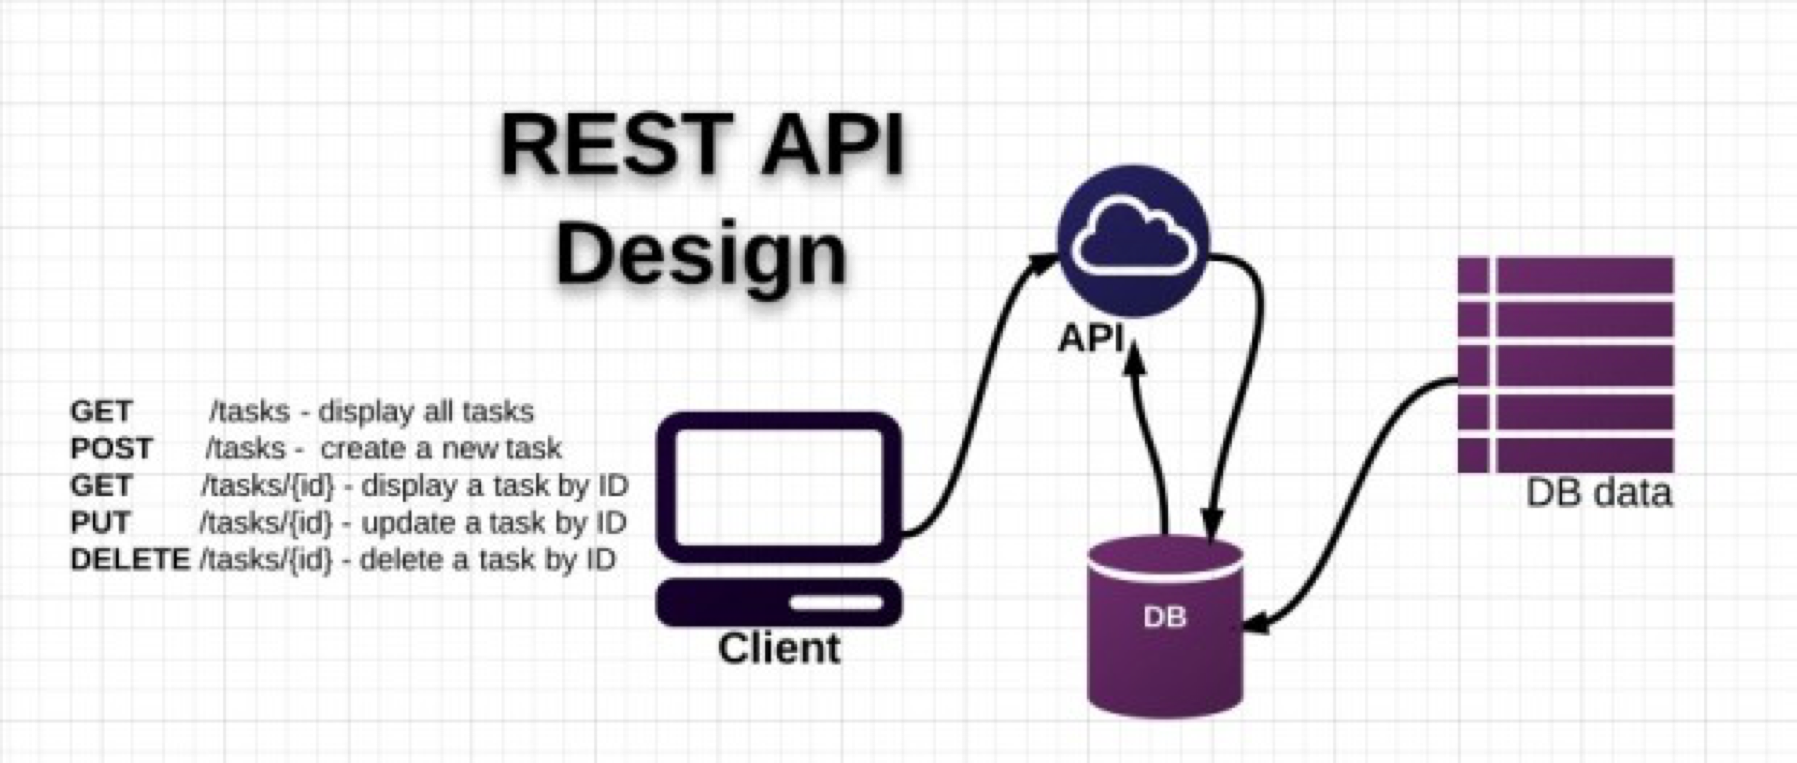
\includegraphics[scale=0.80]{arquitetura}
\caption{Arquitetura REST}
\label{img:arquitetura}
\end{figure}


Ou seja, o sistema se baseia em requisições cliente-servidor. São criados vários módulos seguindo o modelo requisição-resposta, onde no caso do atual projeto cada requisição feita a partir do aplicativo gera uma resposta enviada pelo servidor, a resposta é formatada e mostrada ao usuário de forma visual agradável. Como protocolo de comunicação são utilizados métodos HTTP, principalmente os 4 principais métodos.

\begin{itemize}
\item GET – Utilizado para requisições onde um dado é buscado
\item POST – Utilizado para requisições onde um dado é inserido
\item PUT – Contempla requisições onde um dado é editado
\item DELETE – Aborda requisições onde dados são excluídos

\end{itemize}
	
	Para a utilização do DELETE, optou-se por utilizar a forma de deleção lógica, onde um dado jamais é apagado da base, o que acontece é a utilização de uma flag para indicar que o dado não existe mais. Esse esquema possibilita a criação de um log de alterações e deleções sem a perda de dado algum.
	
\subsubsection{Diagrama de Classes}
O diagrama de classes é a representação da estrutura e relações das classes que servem de modelo para objetos.


\begin{figure}[!htb]
	\centering
	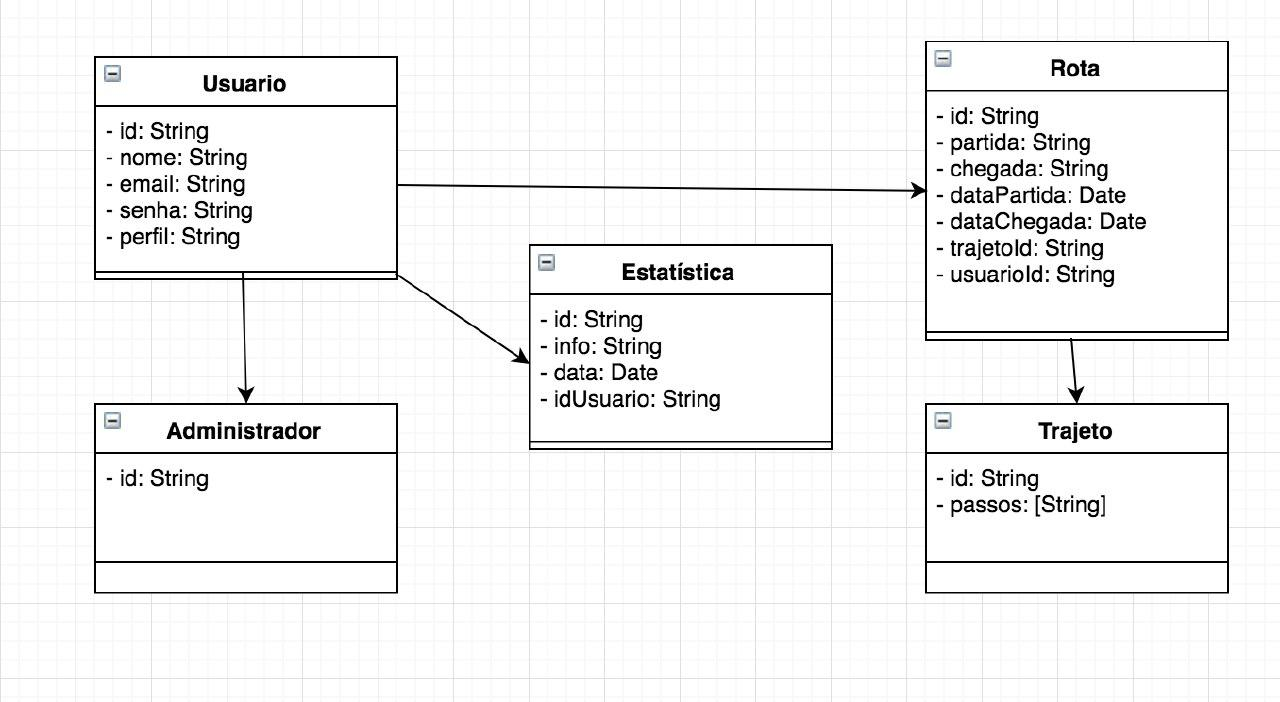
\includegraphics[scale=0.50]{arquitetura_bike.jpg}
	\caption{Diagrama de Classes}
	\label{img:diagramaclasse}
\end{figure}

\subsection{Google Maps API}
Para obter a direção das rotas, será utilizada a API pública do Google Maps, com o benefício de trazer ao aplicativo desenvolvido, toda a precisão de cálculo e processamento encontrado no Google Maps.
O Google disponibiliza uma API pública para a comunicação entre seu servidor e  softwares em geral.

Para a utilização desta API, primeiramente é necessário gerar uma chave de utilização com uma conta de desenvolvedor do Google já existente. Feito isto, basta incluir o script disponibilizado pelo Google, onde for necessária a utilização deste script. 

No caso do atual projeto, será utilizada a API versão 3 que possui algumas funcionalidades como por exemplo a consulta de rotas, em que as versões 1 e 2 da API não possuem.

Para incluir o script da versão 3 basta utilizar o código JavaScript abaixo

\graphicspath{{figuras/}}
\begin{figure}[!htb]
\centering
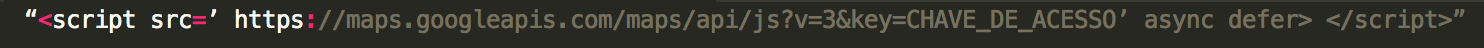
\includegraphics[width=\textwidth]{codigo1}
\caption{Código 1}
\label{img:codigo1}
\end{figure}

Que é completamente compatível com as tecnologias utilizadas no projeto. Observa-se a especificação da versão no primeiro parâmetro da URL, onde v=3. Caso esse parâmetro fosse emitido, o script carregado seria o da versão 1.0 que possui algumas limitações em relação à funcionalidades.

Para a aplicação das funcionalidades, foi produzido um protótipo da utilização da API, para constatar que esta supriria todas as necessidades principais do projeto.

O primeiro passo após a inclusão do Script, foi definir o ponto inicial para cálculo da rota. No protótipo desenvolvido, foi utilizado o meio do ICC no campus Darcy Ribeiro como ponto inicial.

\graphicspath{{figuras/}}
\begin{figure}[!htb]
\centering
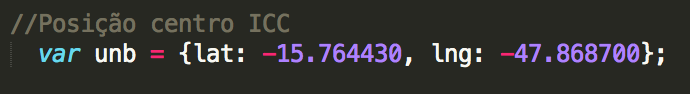
\includegraphics[scale=0.80]{codigo2}
\caption{Código 2}
\label{img:codigo2}
\end{figure}

Em seguida, o objeto mapa foi criado e instanciado na camada de visualização da aplicação.	
	
\graphicspath{{figuras/}}
\begin{figure}[!htb]
\centering
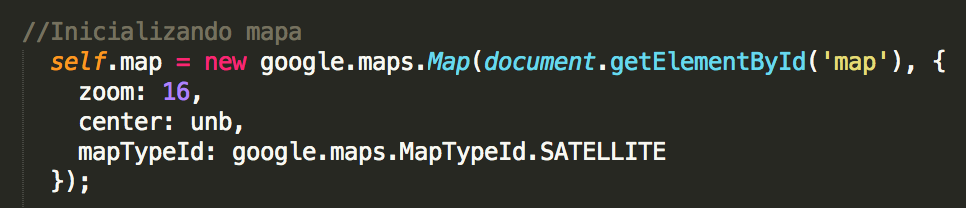
\includegraphics[scale=0.80]{codigo3}
\caption{Código 3}
\label{img:codigo3}
\end{figure}

Ainda foi aplicada uma camada de visualização em cima do mapa, mostrando um mapa detalhado sobre o campus Darcy Ribeiro.

\graphicspath{{figuras/}}
\begin{figure}[!htb]
\centering
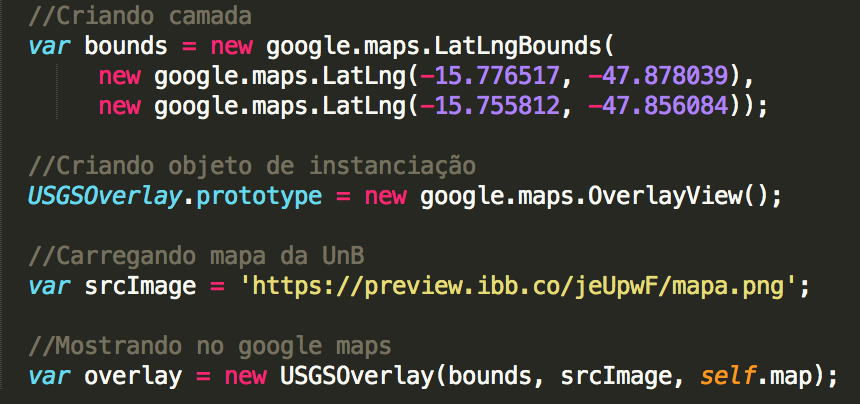
\includegraphics[scale=0.80]{codigo4}
\caption{Código 4}
\label{img:codigo4}
\end{figure}

A seguir foi desenhado um pino, apenas para representar a posição inicial.

\graphicspath{{figuras/}}
\begin{figure}[!htb]
\centering
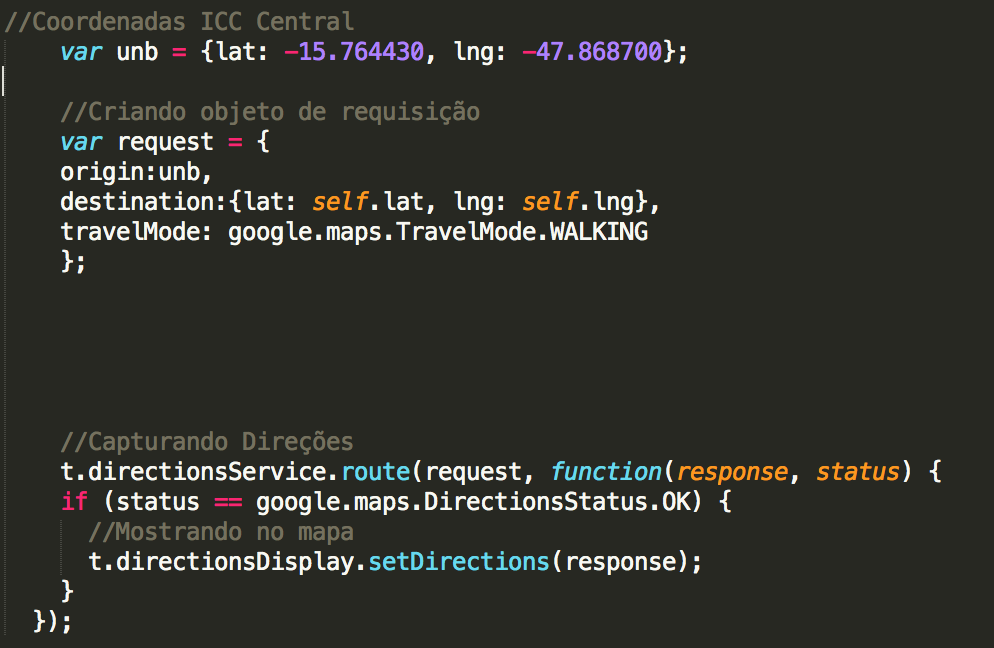
\includegraphics[scale=0.80]{codigo5}
\caption{Código 5}
\label{img:codigo5}
\end{figure}

\newpage

O resultado obtido encontra-se na figura \ref{img:mapa_unb}

\graphicspath{{figuras/}}
\begin{figure}[!htb]
\centering
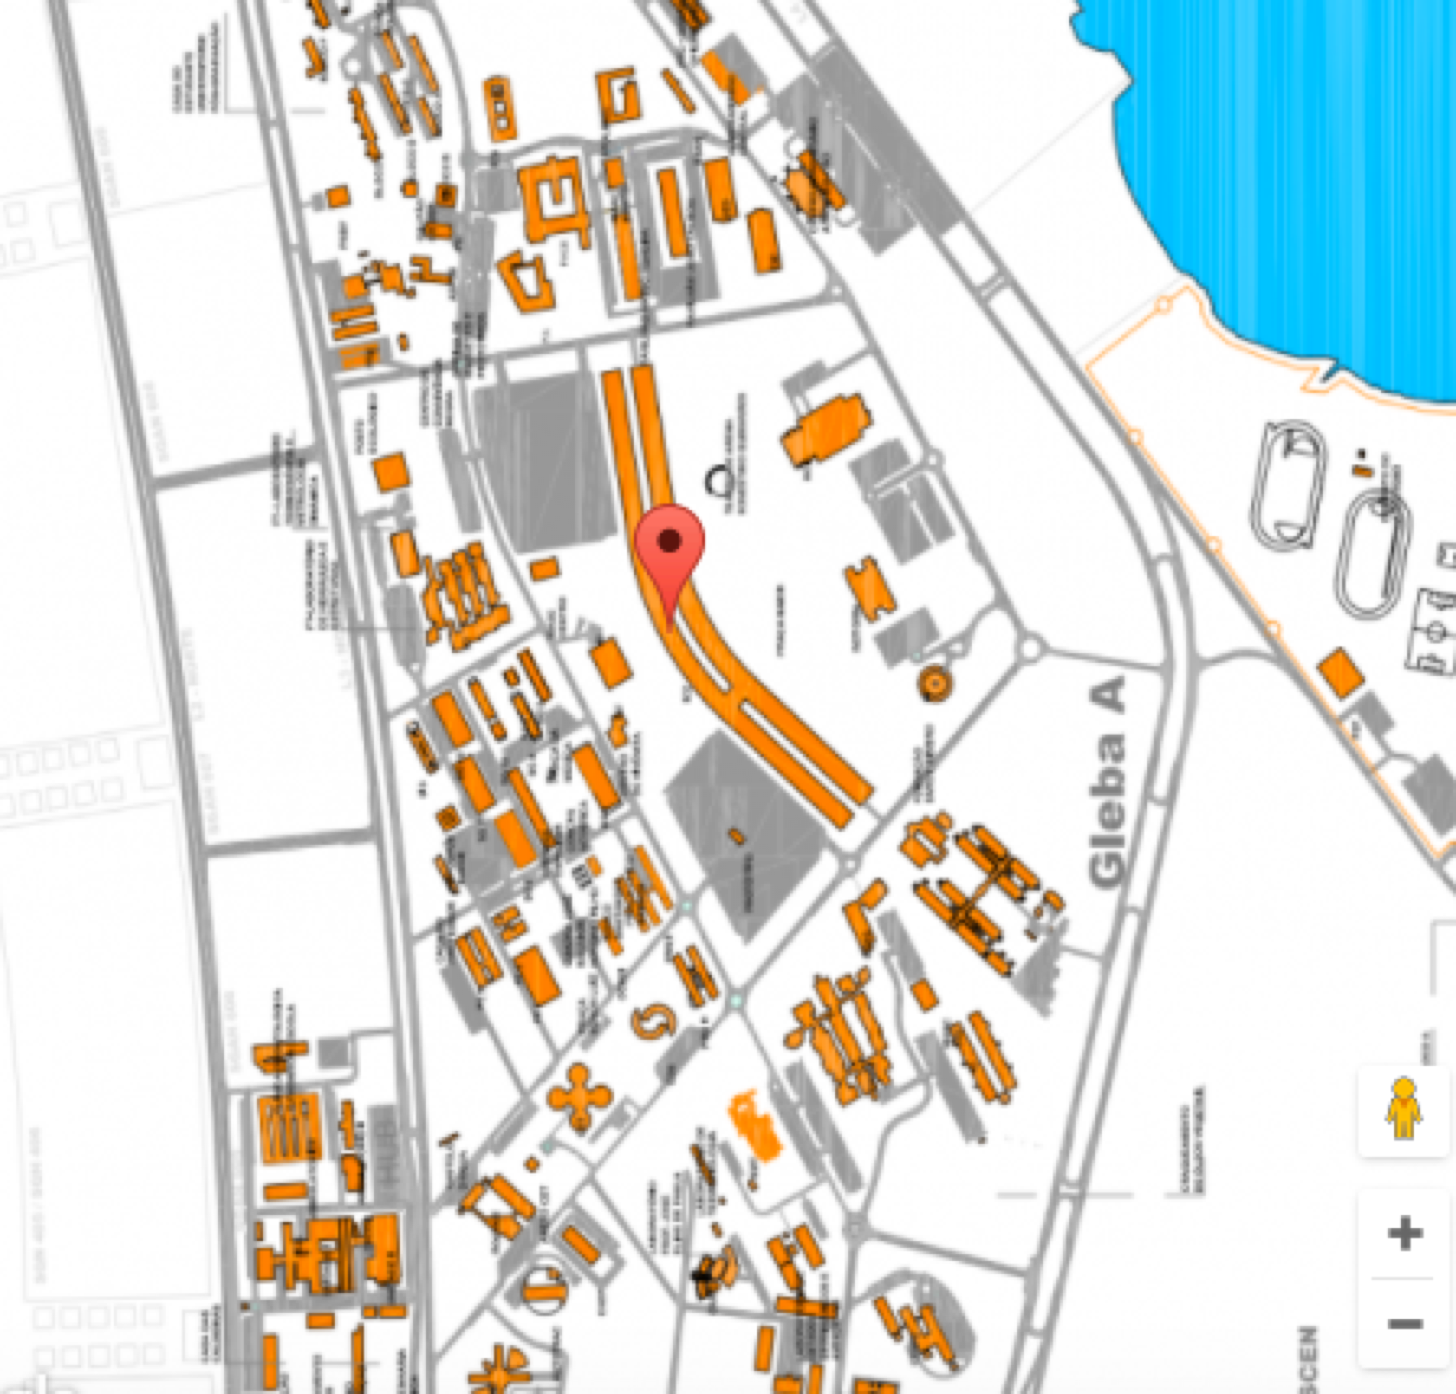
\includegraphics[scale=0.80]{mapa_unb_1}
\caption{Mapa Universidade de Brasília}
\label{img:mapa_unb}
\end{figure}

Os pontos de início e fim são tratados e o serviço de rotas é acionado, retornando um objeto JSON com todos os passos de direções necessários a se chegar no destino desejado.

Cada passo é retornado seguindo um modelo específico, deve-se atentar para a sub-propriedade instructions do array steps. Por exemplo a primeira instrução para ir do ICC ao HUB é ‘Siga na direção Sudoeste em direção a UNB Área 1’. Essas instruções serão passadas por um parser e comunicadas ao micro controlador que se encarregará de comunica-las ao usuário de forma agradável.

No protótipo feito, foi traçada a rota a partir do serviço renderizador, disponibilizado também pela API do Google Maps. O resultado conseguido encontra-se na figura \ref{img:mapa_unb2}, mostrando o traçar de uma rota do ICC ao HUB

\graphicspath{{figuras/}}
\begin{figure}[!htb]
\centering
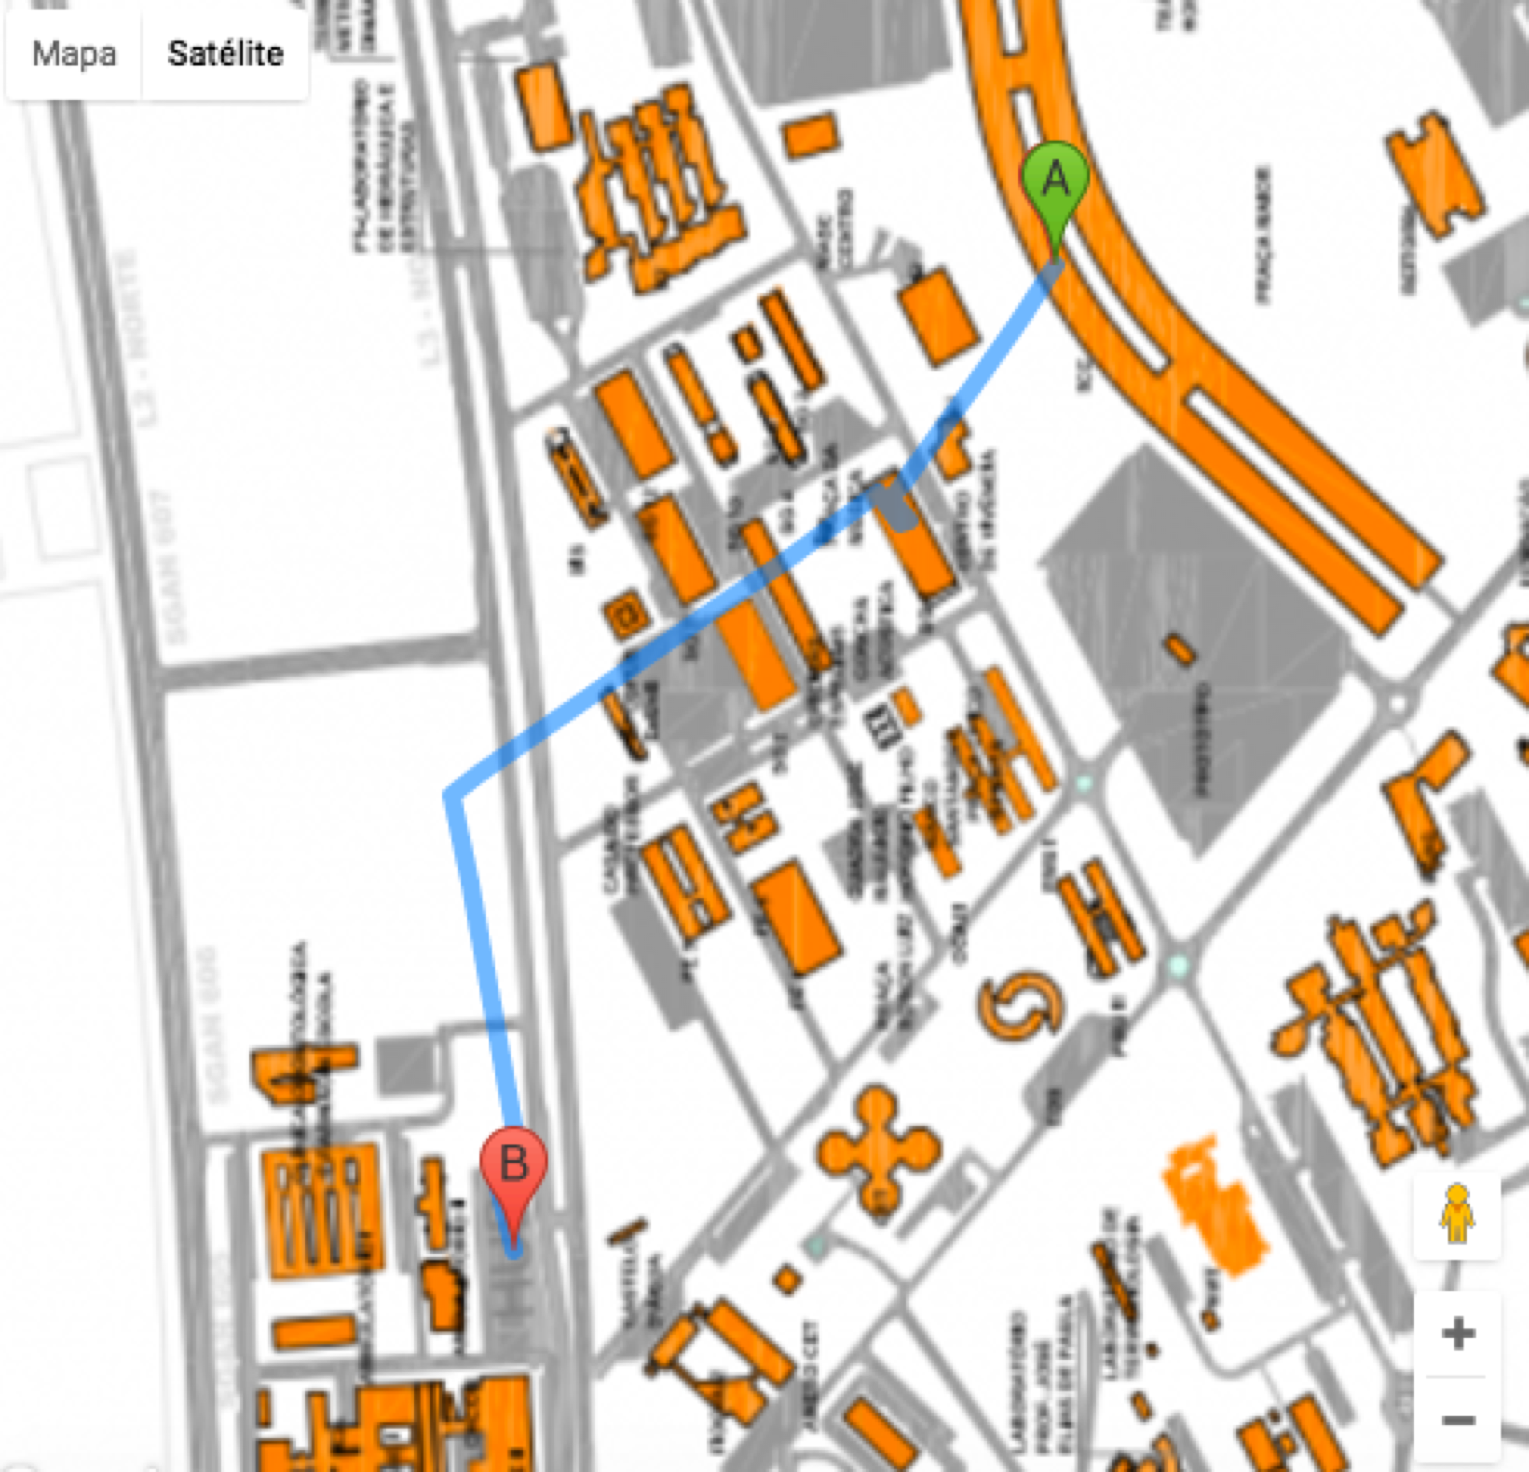
\includegraphics[scale=0.80]{mapa_unb_2}
\caption{Mapa Universidade de Brasília}
\label{img:mapa_unb2}
\end{figure}

\newpage

	\subsection{Protótipo}
	Alguns protótipo das telas foram feitos, para que se possa ter uma noção do produto final que se espera alcançar ao fim do projeto. Os protótipos são apresentados nas figuras \ref{img:logo}, \ref{img:mapa} e \ref{img:dados}.
	
	\graphicspath{{figuras/}}
	\begin{figure}[!htb]
	\centering
	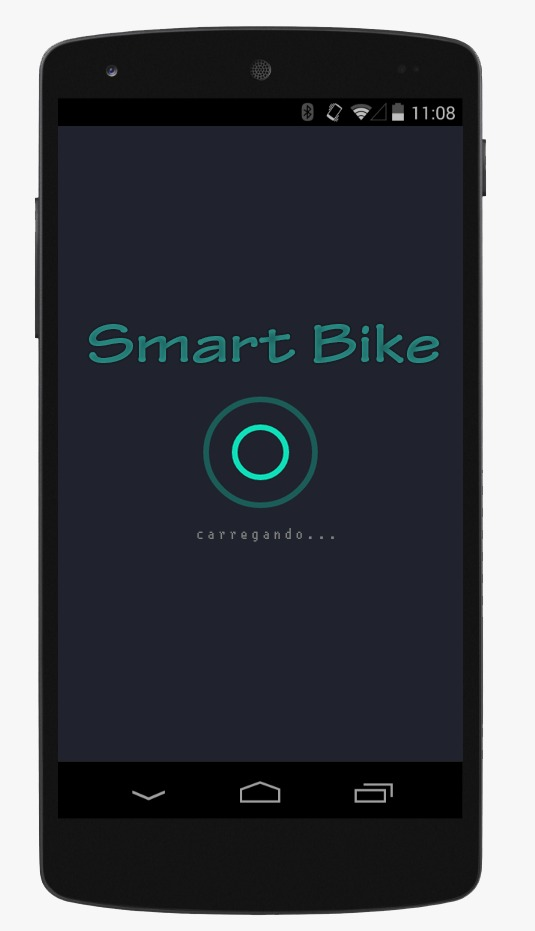
\includegraphics[scale=0.40]{logo.jpeg}
	\caption{Tela de abertura do Aplicativo}
	\label{img:logo}
	\end{figure}

\newpage	

	\graphicspath{{figuras/}}
	\begin{figure}[!htb]
	\centering
	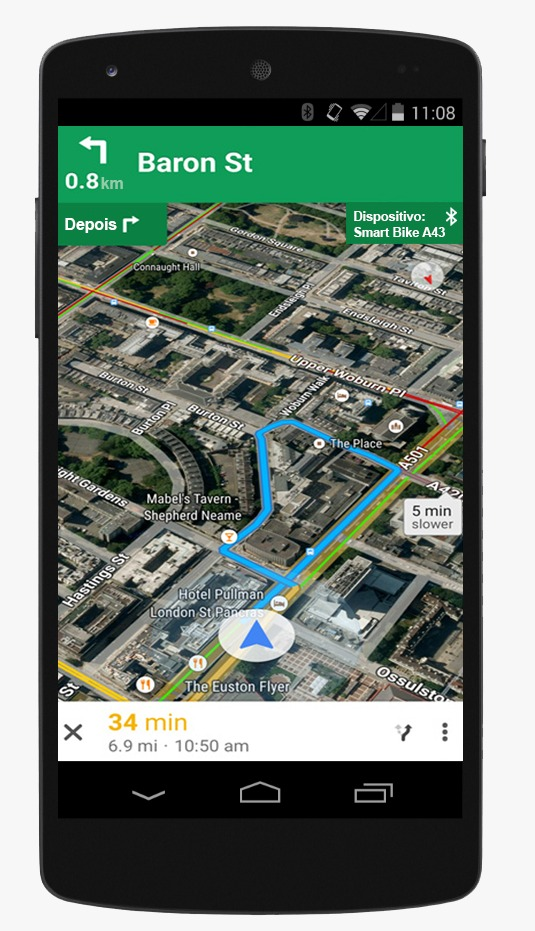
\includegraphics[scale=0.40]{mapa.jpeg}
	\caption{Tela exemplificando o funcionamento do mapa}
	\label{img:mapa}
	\end{figure}
	
\newpage
	
	\graphicspath{{figuras/}}
	\begin{figure}[!htb]
	\centering
	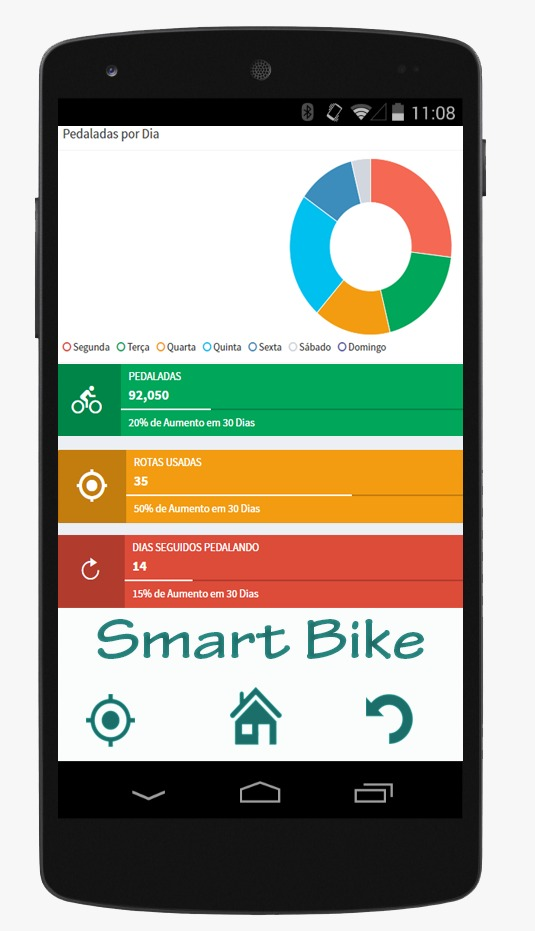
\includegraphics[scale=0.40]{dashboard.jpeg}
	\caption{Tela com os dados do Usuário}
	\label{img:dados}
	\end{figure}
	
	\subsection{Qualidade de Código}
	Para analisar a qualidade do código produzido, foi feito uma análise utilizando a ferramenta Code Climate.
	O Code Climate é uma ferramenta que analisa todos os arquivos do projeto em cada
	alteração, analisando fatores como itens de complexidade, branches, complexidade
	por método, duplicação de código, quantidade de vezes que o arquivo foi modificado e
	quantidade de linhas.
	Foi obtida nota 3.81 de um total de 4.0, pode ser considerada uma nota alta mas
	possível de ser melhorada, também foi adotado o padrão de código de JavaScript mundialmente conhecido do airbnb.
	
	\subsection{Plano de Integração}
	  A comunicação entre o celular e o microcontrolador será feita através de receptor \textit{bluetooth} acoplado ao microcontrolador. Para que seja feita essa comunicação, será utilizada a API do próprio sistema android para troca de informações via \textit{bluetooth}. Dentre os principais recursos que a API fornece, os que mais serão utilizados serão:
	  \begin{itemize}
	  	\item Busca por outros aparelhos \textit{bluetooth};
	  	\item Pareamento entre o adaptador \textit{bluetooth} e o dispositivo\textit{bluetooth};
	  	\item Conexão com \textit{sockets} específicos de outros aparelhos;
	  	\item Transferência de arquivos;
	  \end{itemize}
	  
	  Deve-se ressaltar que para a utilização do \textit{bluetooth} do aparelho é necessário que o dispositivo permita a utilização de tais recursos, sem essa permissão não é possível fazer a comunicação entre os dois dispositivos.  
  	Para realizar a busca do adaptador \textit{bluetooth} que estará instalado na placa microcontroladora será utilizado o seguinte trecho de código apresentado na figura \ref{img:bluetooth_enabled}
  	
  	\graphicspath{{figuras/}}
  	\begin{figure}[!htb]
  	\centering
  	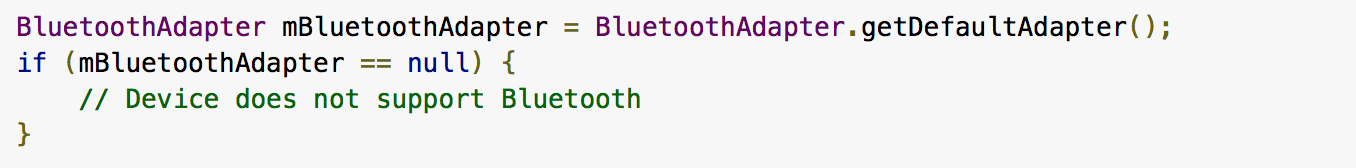
\includegraphics[scale=0.60]{bluetooth_enabled}
  	\caption{Trecho de código exemplificando a comunicação \textit{bluetooth}}
  	\label{img:bluetooth_enabled}
  	\end{figure}
  	
  	Para garantir que o dispositivo \textit{bluetooth} será adicionado apenas uma vez, será utilzado um trecho de código parecido com o da figura \ref{img:bluetooth_devices}, que garante que para um dispositivo ser adicionado ele, não deve estar presente na lista de dispositivos previamente adicionados.
  	
  	\graphicspath{{figuras/}}
  	\begin{figure}[!htb]
  	\centering
  	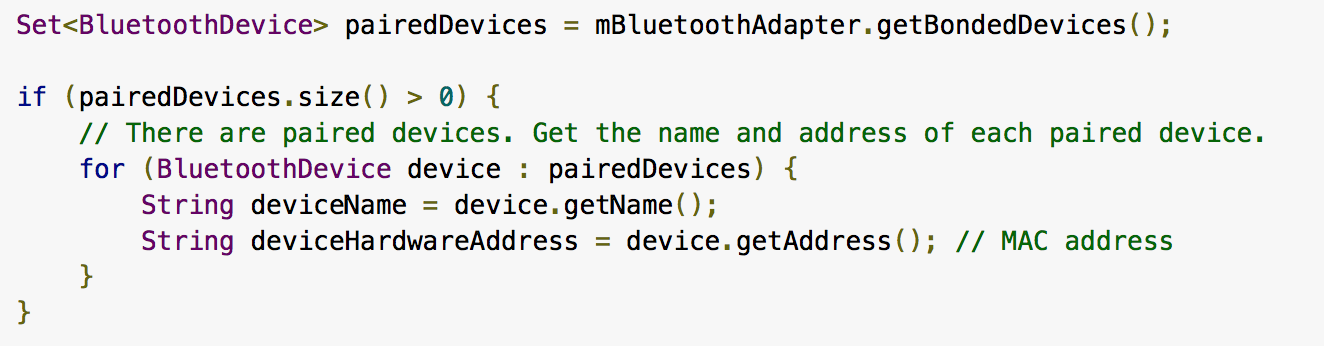
\includegraphics[scale=0.60]{bluetooth_paired_devices}
  	\caption{Trecho de Código que garante que um dispositivo será adicionado apenas uma vez}
  	\label{img:bluetooth_devices}
  	\end{figure}
  	
  	Para que seja feita a transferência de dados entre os dispositivos, o Google (empresa responsável pela documentação da plataforma android), dispõe um trecho de código que serve como guia para implementação desta funcionalidade. Na figura \ref{img:trecho1} é criada uma classe que define as constantes que serão utilizadas ao longo do código.
  	
  	\graphicspath{{figuras/}}
  	\begin{figure}[!htb]
  	\centering
  	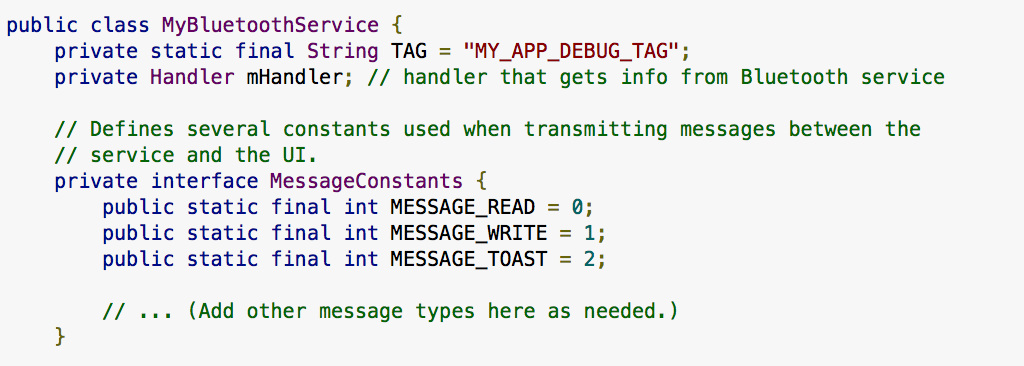
\includegraphics[scale=0.60]{classe_MyBluetoothService}
  	\caption{Neste trecho de código são definidas as constantes que serão utilizadas ao longo do código}
  	\label{img:trecho1}
  	\end{figure}
  
Na figura \ref{img:trecho2} é criada uma outra classe que é a classe que implementa a funcionalidade de troca de dados. Esta classe extende da classe Thread, seus atributos são do tipo \textit{BluetoothSocket}, \textit{InputStream}, \textit{OutputStream} e um \textit{array} de \textit{byte}.

\graphicspath{{figuras/}}
\begin{figure}[!htb]
\centering
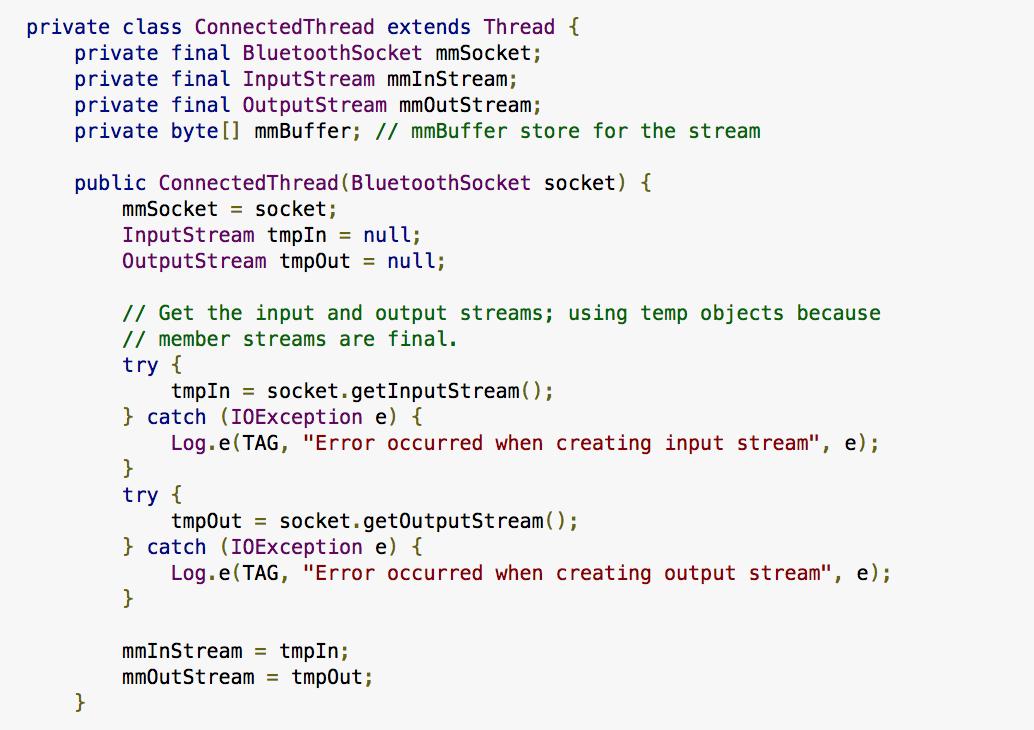
\includegraphics[scale=0.80]{classe_ConnectedThread}
\caption{Nesta classe são implementados os métodos responsáveis pelo funcionamento da troca de dados}
\label{img:trecho2}
\end{figure}

A figura \ref{img:trecho3} apresenta o método \textit{"run"} que funciona em segundo plano constantemente. Este método é responsável por ficar aguardando uma requisição do dispositivo.

\graphicspath{{figuras/}}
\begin{figure}[!htb]
\centering
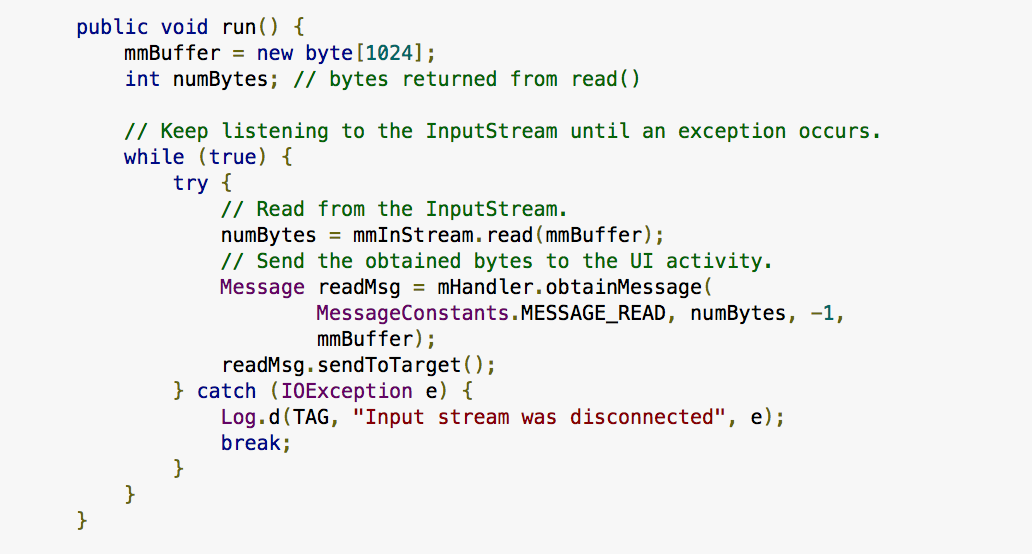
\includegraphics[scale=0.80]{run_method}
\caption{Implementação do método \textit{run} que é responsável por receber as informações do dispositivo \textit{bluetooth}}
\label{img:trecho3}
\end{figure}

O método \textit{"write"} é que faz a escrita dos dados que serão enviados para o dispositivo, como pode ser visto na figura \ref{img:trecho4}.

\graphicspath{{figuras/}}
\begin{figure}[!htb]
\centering
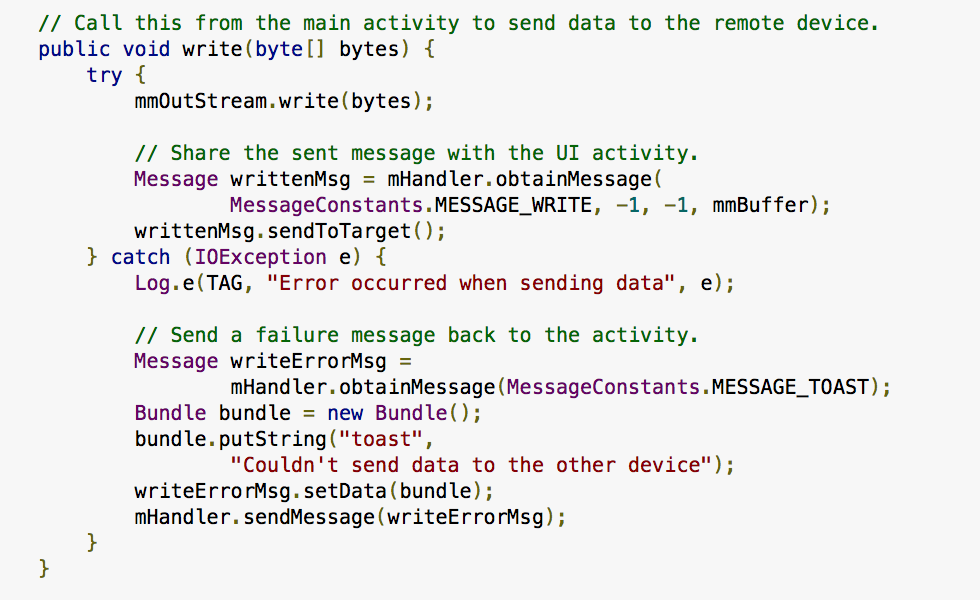
\includegraphics[scale=0.80]{write_method}
\caption{Implementação do método \textit{write} que é responsável por escrever os dados que serão enviados}
\label{img:trecho4}
\end{figure}

Por último, o método \textit{"cancel"} que encerra a conexão com o dispositivo pareado, como mostrado na figura \ref{img:trecho5}

\graphicspath{{figuras/}}
  \begin{figure}[!htb]
  \centering
  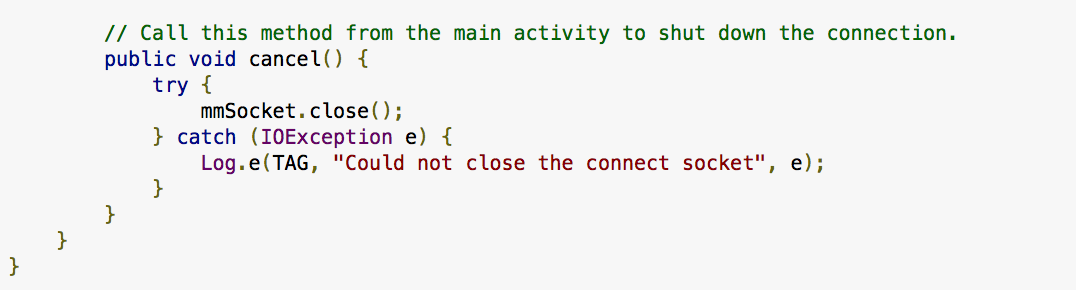
\includegraphics[scale=0.80]{cancel_method}
  \caption{Método \textit{"cancel"} que encerra a conexão com o dispositivo}
  \label{img:trecho5}
  \end{figure}  
  
  \section{Eletroeletrônica}
	
	  	\subsection{Acionamento do Motor}
		\subsubsection{Requisito}
	O sistema de acionamento deve fazer com que o motor gire em velocidade de acordo com a posição do acelerador. Todo o processamento dos dados obtidos pelos sensores hall, localizados no motor, passarão por algoritmos de controle e serão enviados aos transístores de potência. O controle da velocidade será feito utilizando pwm em cada um dos seis transistores. Haverá isolamento elétrico, através de optoacopladores, para proteção do sistema de acionamento.
	\subsubsection{Implementação}
	Será utilizado para prototipagem o microcontrolador arduino.
  
	\subsubsection{Sensores}
	  Os dados sobre a posição do motor são obtidos através de três sensores do tipo hall, localizados dentro do motor.
	
	\subsubsection{Acionamento}
	De acordo com a posição atual, do motor e do acelerador, o sistema ativa o conjunto de optoacopladores, que por sua vez ativarão os transistores de potência gerando torque para movimentar o rotor de acordo com o pwm gerado com base na posição do acelerador.
  
 	 \subsection{Sistema de Controle e Disponibilização dos Dados}
 	\subsubsection{Requisito}
 		Para garantir o bom funcionamento e a estabilidade do conjunto que compõe a bicicleta, é necessário criar um sistema que seja capaz de fornecer ao usuário informações gerais do estado do produto e que oriente o uso do mesmo. Na prática, isso implica em um painel que indica parâmetros como a velocidade exercida pelo veículo, o nível de carga das baterias, a orientação e a distância do percurso.
O sistema inteiro deve ser controlado por um microcontrolador, que receberá os dados dos sensores espalhados pela bicicleta e as ordens provindas do aplicativo e do GPS do celular, transformando tudo em um único sistema integrado e representado por um display acoplado na própria bicicleta. É necessário garantir que esses dados serão filtrados, calibrados e bem estruturados para garantir que os resultados apresentados aos usuários sejam o mais próximo possível da realidade.
	
	\subsubsection{Implementação}
	Para melhor entendimento e análise do microcontrolador, pode-se dividir a função do sistema de controle em duas partes, onde a primeira trata exclusivamente dos sensores e a segunda se refere ao aplicativo.

	\subsubsection{Sensoriamento}
	Existem dois dados a serem coletados através de sensores no sistema, que é a velocidade da bicicleta e o nível de carga das baterias.

Para o controle de velocidade haverá um sensor acoplado na coroa ou nas rodas da bicicleta e este será capaz de enviar sinais com frequências que variam de acordo com a pedalada do usuário. Uma vez que se tenha o dado da frequência é possível processar a velocidade linear instantânea do veículo, que é geralmente dada por v = 2.pi.f.R, onde R é o raio da roda da bicicleta.
Dois tipos de sensores foram levados em consideração para executar essa função. O primeiro deles é o Tacogerador, que funciona como um gerador de corrente contínua onde a sua tensão de saída é proporcional à velocidade do seu eixo. Sua formulação matemática é dada por:
	
	
	Onde: 
	\begin{itemize}
	\item E = F.e.m. gerada na armadura (Volts)
	\item p = Número de pólos
	\item T = Fluxo magnético por pólo (Maxwell)
	\item Z = Número de condutores na armadura
	\item m = Número de percursos na armadura entre os terminais
	\item N = Velocidade (RPM))
	\end{itemize}

	Um Tacogerador comercial têm, em seu datasheet, paramêtros fixos de p, Ø, Z e m. Dessa forma, obtém-se uma relação linear entre a tensão e a velocidade, que é o suficiente para obter a frequência das pedaladas. Essa linearidade tem um "limite de saturação" que varia de acordo com o modelo fabricado. Deve-se levar em consideração os parâmetros aguardados da bicicleta para a escolha do modelo mais adequado.

Outra opção para a captação da frequência é o Encoder, que é um dispositivo eletromecânico que reproduz pulsos elétricos a partir do movimento rotacional do eixo. Trata-se de um sensor de posição, capaz de indicar todas as vezes que um determinado objeto passa por um ponto. Essa característica, somada a uma tomada de tempo, é capaz de definir a frequência da pedalada pela fórmula simples da frequência: f = 1/T. Onde T é o período do movimento da roda.

O uso do Encoder torna a aplicação do sistema viável em qualquer tipo de bicicleta, mesmo não sendo a proposta nesse artigo, uma vez que não é necessário saber dos paramêtros físicos da roda, como o seu raio. Porém, trata-se de um aparato muito maior e mais robusto que o Tacogerador, que demanda mais espaço e mais interferência no sistema geral.

O nível de carga das baterias é um dos pontos mais importantes do produto, por isso o seu controle é fundamental para garantir o funcionamento correto dos motores e do painel. Para aferir esse dado, deve-se entender que a variação de carga em uma bateria interfere em uma variação de tensão e, através de um circuito retificador de tensão, podemos saber em que nível o controle de carga se encontra. Existem diversos modelos que podem ser utilizados nesse projeto, o que vai mudar é a precisão das medidas de acordo com os componentes que serão encontrados e utilizados no circuito.
Pode-se utilizar um conjunto de transistors e diodos para acionar alguns LED's quando uma determinada tensão for alcançada, ou até mesmo um conversor AD para definir algumas faixas de carga a serem apresentadas ao usuário. O espaço físico que poderá ser utilizado e a necessidade da precisão do sistema irão definir qual topologia será utilizada.


\subsubsection{Processamento dos Dados do Aplicativo}
O O aplicativo que integrará o usuário ao sistema será capaz de coletar o caminho que o usuário quer percorrer e, através do GPS do celular, traçar uma rota a ser seguida. Essa rota será constantemente informada ao microprocessador que, através de algum dispositivo, deve orientar o usuário sobre o caminho que ele deve percorrer. Dois parâmetros serão levados em consideração: direção e distância.

O indicador de direção será baseado no modelo clássico de um GPS que contém oito sinais ilustrativos como curvas e curvas suaves, tanto pra direita quanto esquerda, além das direções de rotatórias. Cada desenho  será nomeado com uma palavra de 3 bits, e desenhado com uma estrutura binária de matriz dentro do código. Uma vez que o GPS determinar alguma dessas 8 direções o aplicativo irá dar um comando ao microprocessador, através da palavra de 3 bits, para que o desenho correto de direção seja acionado e apresentado no display. 
Para o melhor entendimento, atribui-se por exemplo a palavra 010 à direção "VIRE A DIREITA". Quando o GPS indicar essa direção, o aplicativo enviará ao microprocessador os níveis de tensão "0", "1" e "0" para o micro, que irá processar a devida imagem no display.

\graphicspath{{figuras/}}
\begin{figure}[h!]
\centering
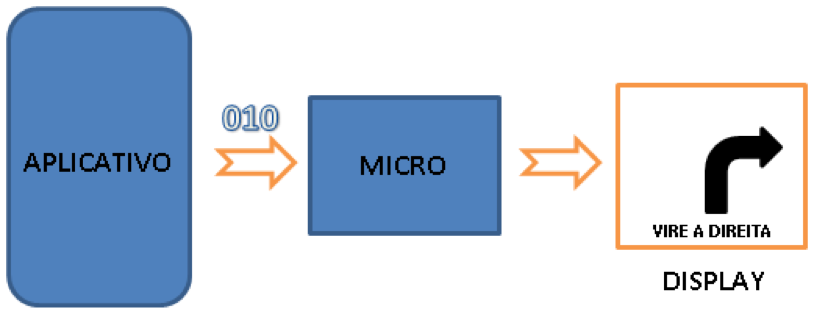
\includegraphics[scale=0.80]{eletronica1.png}
\caption{Eletronica 1}
\label{img:us}
\end{figure}

O envio desses comandos poderá ser feito da forma mais simples, utilizando 3 pinos lógicos de entrada do microprocessador, ou através de uma mensagem serial, que deixa o código mais robusto mas compensa com a economia dos pinos de entrada do sistema.

Para cada direção do GPS nota-se que existe um indicador de distância até que se alcance tal direção. No caso da bicicleta, tais avisos começam a aparecer a partir de uma distância de 50m do ponto em questão. Baseado nisso, o aplicativo também será capaz de enviar essas informações de distância ao microprocessador, que por sua vez irá indicar esses dados ao usuário através do display e de um sinal luminoso.
Uma lâmpada será colocada no painel da bicicleta e, a partir do momento que o GPS indicar informações de distância, ela começará a piscar, aumentando a sua frequência conforme se aproxima do destino. A idéia é que, embora o usuário tenha todas essas informações no display do painel, a sua atenção esteja voltada ao percurso na maior parte do tempo.


Cada desenho desse será nomeado com uma palavra de 3 bits, e desenhado com uma estrutura binária de matriz dentro do código. Uma vez que o GPS determinar alguma dessas 8 direções o aplicativo irá dar um comando ao microprocessador, através da palavra de 3 bits, para que o desenho correto de direção seja acionado e apresentado no display. 
Para o melhor entendimento, atribui-se por exemplo a palavra 010 à direção "SIGA EM FRENTE". Quando o GPS indicar essa direção, o aplicativo enviará ao microprocessador os níveis de tensão "0", "1" e "0" para o micro, que irá processar a devida imagem no display.

\subsubsection{Integração com Sistema de Controle}
Uma vez que o sistema coletou os dados provindos da bicicleta e do aplicativo, será possível processar essas informações e alimentar o painel do usuário, conforme ilustrado a seguir:


\graphicspath{{figuras/}}
\begin{figure}[h!]
\centering
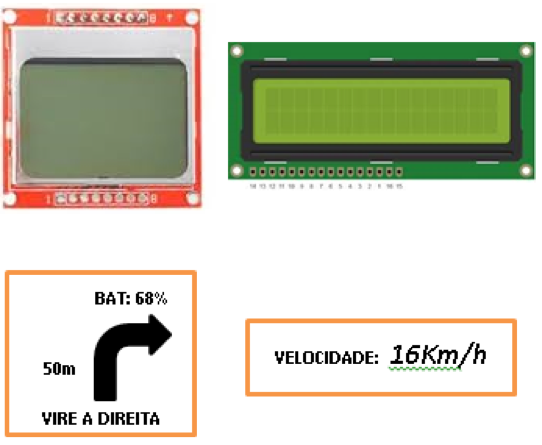
\includegraphics[scale=0.80]{eletronica2.png}
\caption{Eletronica 2}
\label{img:us}
\end{figure}

\subsection{Integração do Circuito}
De acordo com o que é proposto pela parte de acionamento do motor e pela parte do sistema de controle, chega-se a um esboço do diagrama do circuito eletrônico completo do sitema:

Esse projeto, somado com uma fonte de tensão e retificação, definirá o circuito eletrônico final do projeto a ser desenvolvido pelo software EAGLE de circuitos impressos.

  \section{Alimentação}
  A bicicleta elétrica utilizará dois sistemas de alimentação, que serão:
  \begin{itemize}
  	\item Banco de baterias para alimentar o motor elétrico;
  	\item Dínamo para carregar uma bateria que alimentará os componentes eletrônicos e todo o sistema de iluminação do GPS. 
  \end{itemize}
  
	O sistema de navegação será alimentado por um sistema separado do motor elétrico como forma de garantia de suprimento de energia para esse sistema. Caso a bateria descarregue no meio do percurso, o dínamo será capaz de carregá-la enquanto o ciclista pedala a bicicleta, garantindo que o mesmo continuará com o sistema de iluminação que lhe indicará a rota desejada.
	
	\subsection{Motor Elétrico}
De modo geral, pode-se dizer que um motor elétrico é qualquer aparelho ou equipamento que permita transformar energia elétrica em mecânica. Em termos práticos, é amplamente utilizado para diversos fins devido a características que lhe conferem vantagens em relação a outros motores, sendo interessante destacar: o custo baixo da energia que utiliza o fácil transporte devido à massa relativamente baixa que possui, além da versatilidade de adaptar-se a diversos tipos de cargas com características distintas.

Os motores elétricos podem ser divididos em dois grandes grupos, baseados no tipo de corrente que utilizarão em seu processo de transformação de energia: os de corrente contínua (CC) e os de corrente alternada (CA). Na figura \ref{img:tipos_motores}, os diversos tipos de motores elétricos são apresentados para fins de curiosidade e entendimento geral da quantidade de motores possíveis que existem no mercado.	

\graphicspath{{figuras/}}
\begin{figure}[h]
\centering
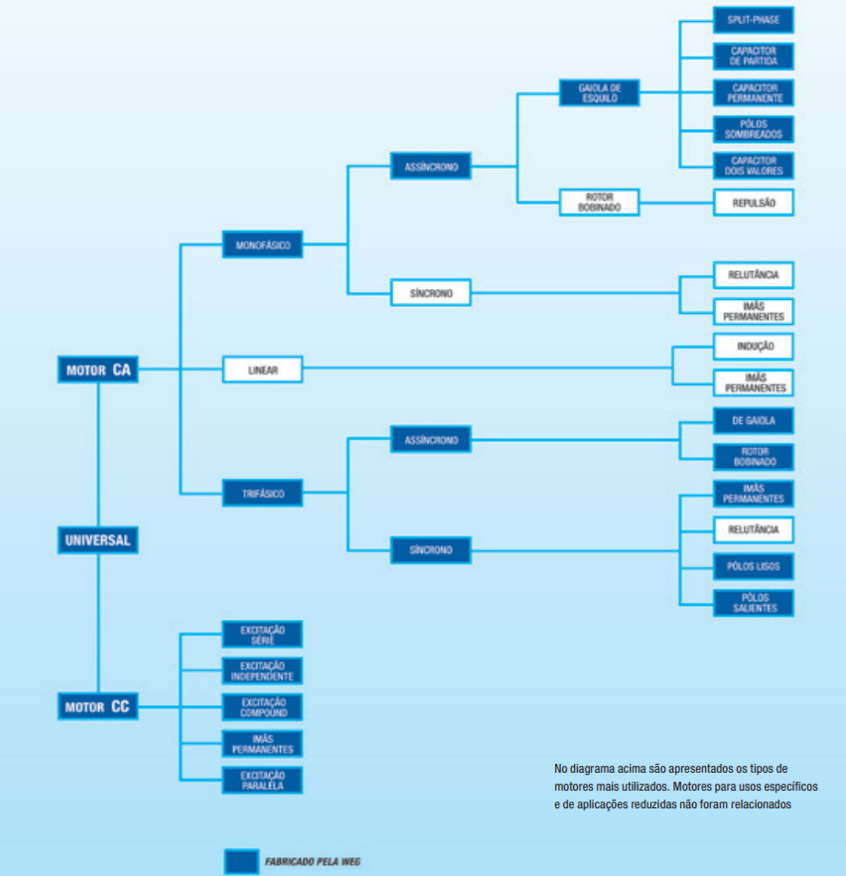
\includegraphics[scale=0.80]{tipos_motores.png}
\caption{Tipos de Motores Elétricos}
\label{img:tipos_motores}
\end{figure}

Apesar da grande variedade de motores, eles possuem características específicas que se adequam melhor a cenários distintos de uso, mesmo que em certos casos possam ser intercambiáveis nos processos, de acordo com as necessidades que a utilização exigirá. Baseando-se nisso, os motores de corrente contínua, os de indução, excitação por imas permanentes e relutância, são os mais utilizados para o uso em bicicletas elétricas.

Os motores elétricos possuem funcionamento baseado na troca de polaridade periódica entre os elementos magnéticos internos, permitindo assim que um rotor possa girar entre dois ímãs e gerar o movimento. Entretanto, a corrente contínua usada em motores CC é interessante para polos permanentes, fazendo com que seja necessária uma inversão do sentido da corrente a cada vez que os polos do rotor se encontrem com os dos ímãs. Para produzir esse efeito, geralmente usam-se comutadores, que são basicamente placas que envolvem o rotor, associada a outro elemento, chamado de escova, assim quando a corrente “entra” no sistema, ela tem seu caminho passando pela escova, parede do comutador, rotor, parede do outro comutador e a outra escova, onde ela inverte a polaridade, voltando para a fonte. 
 
 Considerando quanto ao uso ou não das escovas para o processo explicitado, os motores de corrente contínua podem ser divididos em dois subgrupos: com escovas e sem escovas. Aqueles que possuem as escovas tem seu funcionamento como já citado, já aqueles que não possuem ainda mantem o mesmo modo de obtenção do movimento do motor a partir da posição, entretanto, realizam a comutação eletronicamente, por meio de sensores que indicam o posicionamento instantâneo do motor. 

No caso apresentado neste relatório, o motor, já cedido anteriormente e que será aproveitado nesse projeto, é um motor de corrente contínua sem escovas. No quadro \ref{esp_motor} são apresentados alguns poucos dados apresentados pelo vendedor do motor em relação a características do mesmo. Os demais dados não foram oferecidos pelo site mesmo após tentativa de contato, tornando escassos os dados. Além da tabela, na figura \ref{img:motor} têm-se uma imagem do motor.

\begin{table}[h!]
\centering
\caption{Especificações do Motor}
\label{esp_motor}
\begin{tabular}{|l|}
\hline
Especificações Motor Wind Bikes \\ \hline
Tração: Traseira                \\ \hline
Massa: 5,710 kg                 \\ \hline
Sistema de 120 graus            \\ \hline
\end{tabular}
\end{table}

\graphicspath{{figuras/}}
\begin{figure}[h!]
\centering
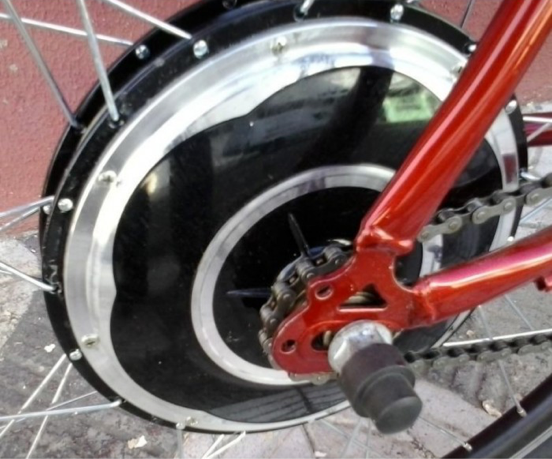
\includegraphics[scale=0.80]{motor.png}
\caption{Motor \textit{Wind Bikes}}
\label{img:motor}
\end{figure}
	
	\subsection{Dínamo}
	Gerador elétrico é uma máquina capaz de converter energia mecânica em energia elétrica, baseado no princípio físico de indução magnética \cite{maximo}. O dínamo é um tipo de gerador elétrico e foi primeiramente utilizado em bicicletas em 1896, patenteado por Alfred Rodriguez. Um dínamo típico utilizado em bicicletas pode ser visto na Figura \ref{img:dinamo_bicicleta}.
	
	\graphicspath{{figuras/}}
	\begin{figure}[h!]
	\centering
	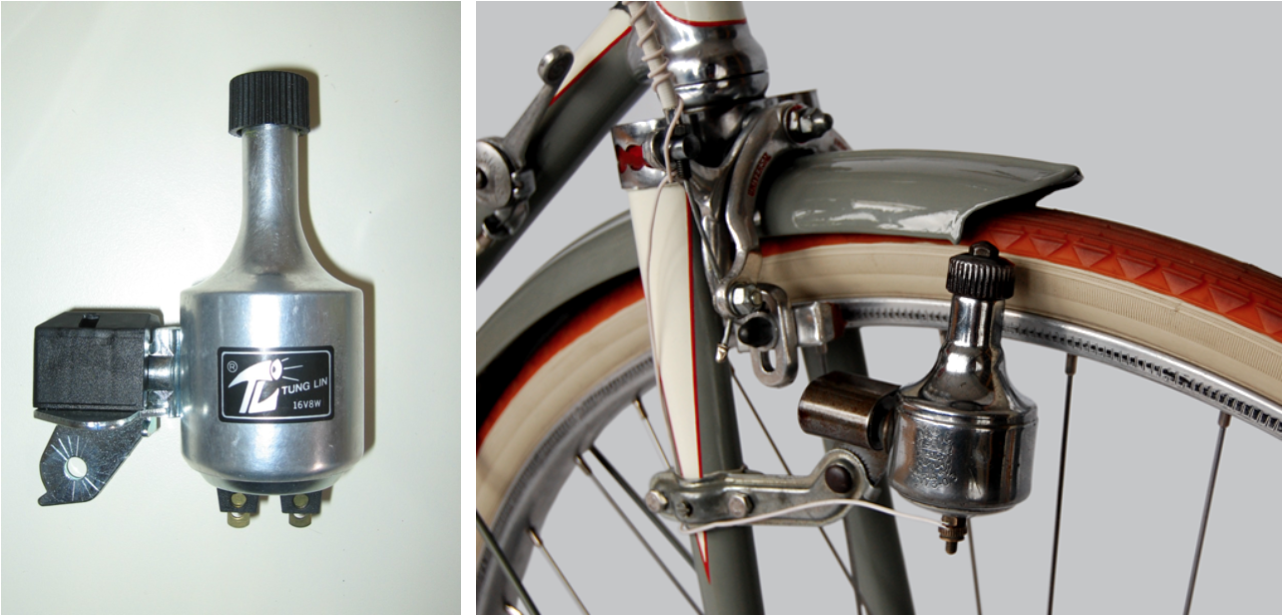
\includegraphics[scale=0.60]{dinamo_bicicleta}
	\caption{Dínamo de Bicicleta}
	\label{img:dinamo_bicicleta}
	\end{figure}
	
Acoplado à roda da bicicleta, o dínamo utiliza a energia cinética de rotação da roda girando um íma que excitará as bobinas circundantes gerando corrente elétrica, que será retificada e irá carregar a bateria por meio de cabos. A bateria irá, então, alimentar os componentes eletrônicos como o microcontrolador e as placas de LED.

A potência mecânica é dada pelo produto do torque () e da velocidade angular () da roda da bicicleta, como visto na Figura \ref{img:potencia_mecanica}. 

\graphicspath{{figuras/}}
\begin{figure}[h!]
\centering
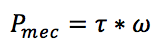
\includegraphics[scale=1.0]{potencia_mecanica}
\caption{Fórmula de potência mecânica}
\label{img:potencia_mecanica}
\end{figure}

Sendo que o torque é dado pela equação da figura \ref{img:torque}, onde r é o raio da roda

\graphicspath{{figuras/}}
\begin{figure}[h!]
\centering
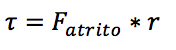
\includegraphics[scale=1.0]{torque}
\caption{Fórmula para cálculo do torque}
\label{img:torque}
\end{figure}


As velocidades serão medidas experimentalmente com o uso de um tacômetro e a tensão e corrente de saída do dínamo com um multímetro.

Apesar de nesse projeto definirmos o conceito de dínamo, a aplicação do mesmo nao existirá, haja vista a exigência dos professores da disciplina que o projeto conseguisse fazer com que o motor elétrico em si conseguisse atuar como gerador e basicamente fizesse a função que o dínamo teria, de maneira mais eficiente e exigindo um grau maior de conhecimento para a realização. Assim, esse tópico está no relatório apenas para fins de demonstração do aperfeiçoamento do projeto e registro das ideias iniciais. 
  
\subsection{Bateria}
	Baterias são dispositivos capazes de converter energia química em energia elétrica através de reações de oxirredução. Ao ligar dois componentes químicos de polos opostos, anodo e catodo, uma diferença de potencial é gerada e elétrons migram do polo negativo, anodo, para o polo positivo, catodo, gerando, assim, uma corrente elétrica. Algumas também são capazes de fazer o processo inverso, convertendo energia elétrica em energia química. Dessa forma, as baterias são usadas como uma fonte de energia elétrica e como armazenamento dessa energia \cite{varela}.
	
	Os tipos de bateria mais utilizadas são: chumbo-ácido, níquel-metal hidreto e íon-lítio.
	
	\begin{itemize}
		\item \textbf{Chumbo-Ácido}: São as baterias com maior maturação no mercado por serem utilizadas há mais tempo, apresentam baixo custo e confiabilidade, sendo muito utilizadas para partidas de motores de automóveis, iluminação, ignição e tração. Sua densidade de energia e energia específica, porém, são a de menor valor \cite{bezerra}.
	\item \textbf{Íon-Lítio}:  São baterias mais leves, com alta densidade de energia, maior eficiência energética que as demais e elevado número de ciclos de vida. O custo é ainda muito alto e a tolerância a sobrecarga é baixa correndo riscos de danificação \cite{bezerra}. São muito utilizadas em aparelhos eletrônicos como celulares e laptops.
	\end{itemize}
	
	A capacidade de uma bateria é dada pela equação da figura \ref{img:calculo_bateria}
	
	\graphicspath{{figuras/}}
	\begin{figure}[h!]
	\centering
	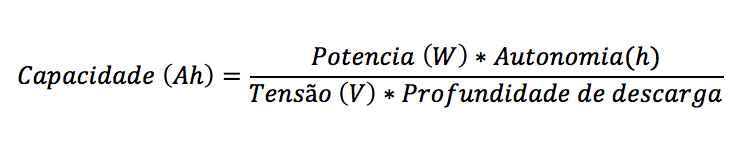
\includegraphics[scale=1.0]{capacidade_bateria}
	\caption{Fórmula para cálculo da bateria}
	\label{img:formula_capacidade}
	\end{figure}
	

	%\citeonline{daanalise} coletou informações sobre rotas cíclicas mais escolhidas por ciclistas quando usando GPS. Em seus resultados, os percursos mais longos feitos duravam, em média, 20 minutos e os participantes da pesquisa faziam, em média, 2,5 viagens por dia. Os percursos totais, por dia, para cada ciclista, duram, em média, 50 minutos. Para dimensionar a bateria, portanto, considera-se o motor trabalhando em máxima potência e o tempo de autonomia de 1h.
	
	\graphicspath{{figuras/}}
	\begin{figure}[h!]
	\centering
	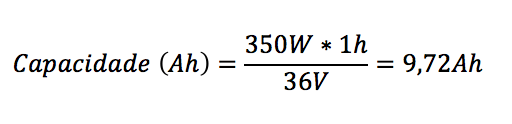
\includegraphics[scale=1.0]{calculo_capacidade}
	\caption{Cálculo da bateria a ser utilizada}
	\label{img:calculo_bateria}
	\end{figure}
	
	Portanto, para alimentar o motor, serão utilizadas três baterias chumbo-ácido de 12V cada, ligadas em série, com capacidade de 10Ah. A escolha desse tipo de bateria foi escolhida devido ao menor custo e maior disponibilidade por ser uma tecnologia mais madura para aplicações automotivas.

	A demanda de corrente típica de cada componente eletrônico segue listado abaixo:
	
	\begin{itemize}
		\item \textbf{Microcontrolador}: 40mA por pino. Um arduíno possui 14 pinos, supondo que sejam usadas todas as entradas, o arduíno demandará 700mA.
		\item \textbf{Microprocessador}: 50A.
		\item \textbf{LED}: 20mA cada.

	\end{itemize}

Os componentes demandam uma corrente de 800 a 900mA. Será utilizada uma bateria de 12V e 1,3Ah que o grupo já possui.

Inicialmente, o cálculo da capacidade da bateria forneceu uma estimativa de qual seria a autonomia dimensionada para todo o sistema. Entretanto, posteriormente, a questão de manter uma autonomia maior foi posta de lado em prol dos custos e do fato de que nesse projeto integrador o objetivo principal é o de funcionamento e integração dos sistemas, não necessariamente de toda a usabilidade completa e já comercial para o usuário, permitindo assim que uma autonomia menor pudesse ser adotada para conter parte dos custos, visto que um conjunto de baterias de 12V de tensão e 10ah de capacidade nominal em um ensaio C1 ou C5 teriam um custo quatro vezes maior quando comparada a baterias comerciais mais simples, ainda de 12V de tensão, porém com apenas 7ah de capacidade nominal em teste C20. Os ensaios e as nomenclaturas CX referem-se aos testes feitos com as baterias pelas próprias empresas para verificar o quanto de corrente a bateria consegue descarregar ao longo do tempo, onde C1 é uma hora, C5 seriam cinco horas e C20, vinte horas. Assim, uma bateria de 10Ah C1, consegue descarregar 10A em uma hora. Já a bateria escolhida, de 7Ah C20, consegue apenas 7A em vinte horas.

As baterias escolhidas pelo grupo foram três do modelo 12MVA-7 Nobreak da Moura, uma bateria usada para aplicações como cercas elétricas, portões elétricos e também em algum grau para bicicletas elétricas e outras aplicações mais simples. A imagem x apresenta uma foto da bateria, enquanto a imagem x+1 traz especificações desta retiradas do catálogo da Moura.

	\begin{figure}[!htb]
		\centering
		
\includegraphics[scale=0.5]{bateria_bike.jpeg}
		\caption{Foto da Bateria Moura 12MVA-7 Nobreak}
		\label{img:bateriabike}
	\end{figure}
	
	\begin{figure}[!htb]
		\centering
		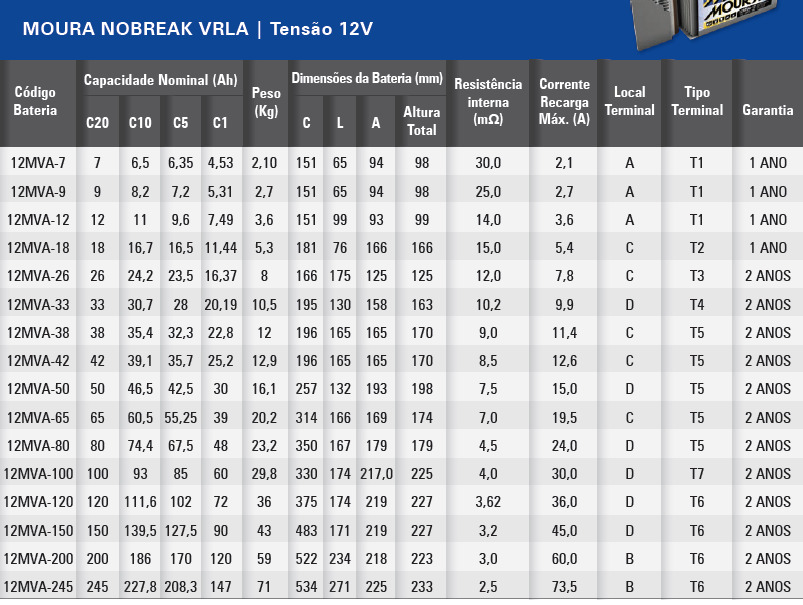
\includegraphics[scale=0.5]{especificacao_bateria.jpeg}
		\caption{Especificações Bateria 12MVA-7}
		\label{img:especificacaobateria}
	\end{figure}
	
Como as especificações apresentam, as baterias serão capazes de suprir a demanda de corrente do sistema e dos componentes eletrônicos, visto que agora não haverá mais outra bateria para suprir somente os componentes menores, exigindo que apenas o banco de três de baterias alimente todo o conjunto, motor e equipamentos eletrônicos. Como dito anteriormente, a autonomia não foi considerada um requisito, mas é seguro afirmar que ela será inferior a uma hora, o tempo proposto inicialmente.

\subsubsection{Circuito de Carregamento da Bateria}
Um carregador, como o nome já dá uma ideia, é basicamente um dispositivo capaz de recarregar outro componente específico, nesse caso, as baterias. Como as baterias de chumbo-ácido possuem alguns critérios básicos para que não afetem a qualidade da bateria, tornando sua vida útil menor. Um deles é a necessidade de o carregamento ser feito com as baterias ligadas em paralelo entre elas, além de ser interessante para a preservação dela que a corrente de carregamento não ultrapasse 10\% da capacidade nominal que a bateria possui. No caso específico da nossa bateria, de capacidade 7Ah, essa corrente seria 0,7 A. 
A partir disso, com uma fórmula bem simples, é possível estimar o tempo de carregamento total da bateria:

\textbf{\centering TR = C/i}

Onde TR seria o tempo de recarga, C a capacidade nominal e i a corrente. 
Em um cálculo rápido é possível observar que o tempo de recarga das baterias seria de aproximadamente 10 horas. 
Procurando em diversos repositórios de circuitos, foi possível encontrar um circuito específico que aparenta atender as necessidades que o projeto exige e que serviria de base para conseguirmos fazer um próprio, adaptado ao fato de ser necessário carregar três baterias em conjunto e não apenas um como no exemplificado. O circuito também se apresenta como uma alternativa interessante, pois utiliza o que, segundo Destro, seria a maneira ideal de recarregar uma bateria de chumbo-ácido de 12 V. 
Essa forma ideal de carregamento consiste em três “fases” de carregamento: uma fase de recarga, onde se eleva a tensão da bateria até 13,8 V, seguida de uma fase de equalização, onde as células das baterias atingem a tensão limite e por fim uma fase de flutuação, onde a tensão é reduzida para a faixa de flutuação da bateria, geralmente 13,2 a 13,8 V, em baixa corrente. Na figura x+2 é apresentado as três etapas de carregamento tidas como ideais.

	\begin{figure}[!htb]
		\centering
		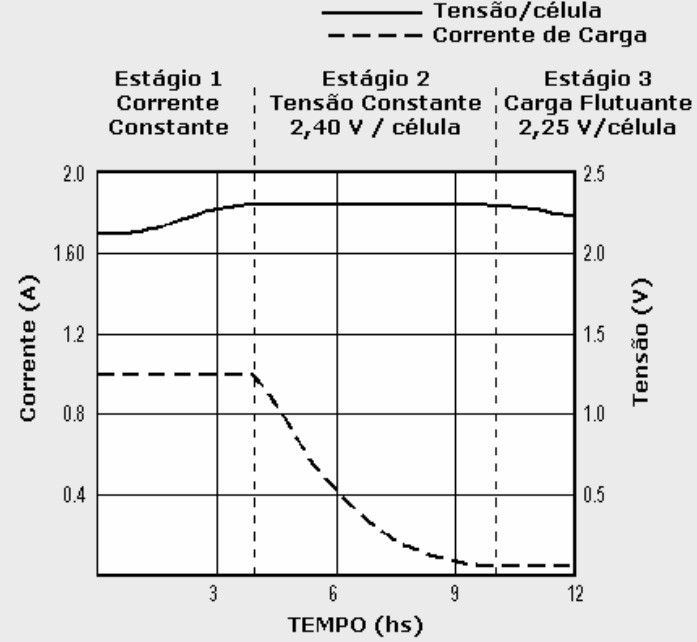
\includegraphics[scale=0.5]{estagio_carregamento.jpeg}
		\caption{Estágios de Carregamento Bateria Chumbo-Ácido}
		\label{img:estagiocarregamento}
	\end{figure}

O circuito retirado proposto pelo site Destro é apresentado na figura x + 3.

	\begin{figure}[!htb]
		\centering
		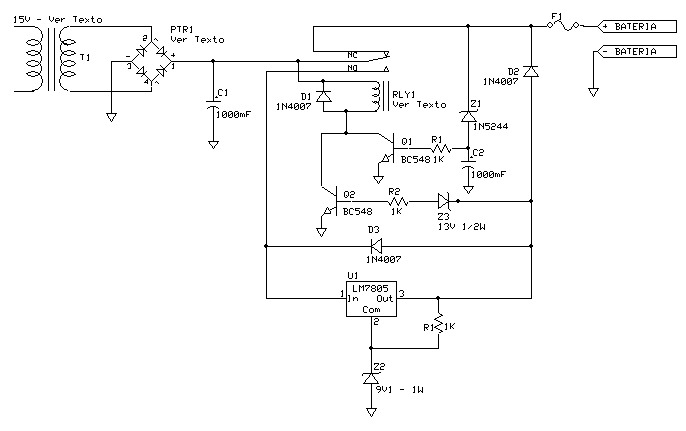
\includegraphics[scale=0.5]{circuito_carregamento.jpeg}
		\caption{Circuito de Carregamento de Referência}
		\label{img:circuitocarregamento}
	\end{figure}
  
  \section{Estrutura}
  Este projeto visa a construção de uma bicicleta elétrica capaz de seguir uma rota pré-determinada via gps. Porém, há a necessidade de se projetar com a devida atenção toda a estrutura da bicicleta de modo que os demais componentes sejam devidamente adaptados de forma ergonômica, em outras palavras, maximizar a segurança e eficiência da interação máquina e ser humano.
Foram levados em consideração vários fatores, como o material, a estabilidade, conforto e custo-benefício para a escolha e dimensionamento da estrutura.O quadro da bicicleta guardará os motores, baterias e demais componentes eletroeletrônicos de forma segura e organizada. Haverá também, um painel bastante intuitivo que auxiliará o usuário em sua rota como: indicação da bateria restante, distância percorrida e distância restante.
	
	\subsection{Materiais}
	Dentre os materiais que compõem o quadro da bicicleta, foi se escolhido o alumínio, por se tratar de um material leve, barato, com ponto de fusão suficientemente seguro para ser integrado com os componentes eletroeletrônicos além da pouca oxidação sofrida. Outros materiais que foram pesquisados com a finalidade de implementação, foram o aço, porém possui um peso elevado se comparado ao alumínio, e está sujeito a oxidação, apesar do baixo preço. Fibra de carbono, possui um baixo peso, porém um alto custo e uma grande dificuldade na parte de manutenção e conserto.
	
	\subsection{Ergonomia}
	Atualmente no mercado brasileiro as bicicletas mais vendidas são as Mountain Bike, comumente apelidadas de MTB. Isso se deve a sua versatilidade que permite ser utilizada em qualquer terreno. Elas geralmente são encontradas nos tamanho de quadro 17, 18 e 19”. Os dois primeiros tipos são indicados para pessoas entre 1,68 e 1,78 metros de altura enquanto a última atende a faixa de 1,78 e 1,85 metros. 
Segundo a pesquisa de orçamentos familiares realizada pelo IBGE entre 2008 e 2009, a estatura média da mulher e do homem brasileiro adulto são, respectivamente, 1,71 e 1,60 metros. Associando esse dado com os tamanhos de quadros mais comuns do mercado optou-se por utilizar como base para o projeto um quadro de 17”.  
As análises ergonômicas serão realizadas com o auxílio do software CATIA V5 utilizando sua base de dados referente ao estudo de percentil do norte americano. Para o problema apresentado serão adotadas as medidas dos homens de percentil entre 13 e 65, e para mulheres entre 79 e 99, ambos norte americanos.

	\subsection{Design}

	O \textit{design} da bicicleta é apresentado na figura \ref{img:dimensoes}, onde é possível ver as dimensões da bicicleta a ser produzida.	
	
	\graphicspath{{figuras/}}
	\begin{figure}[h!]
	\centering
	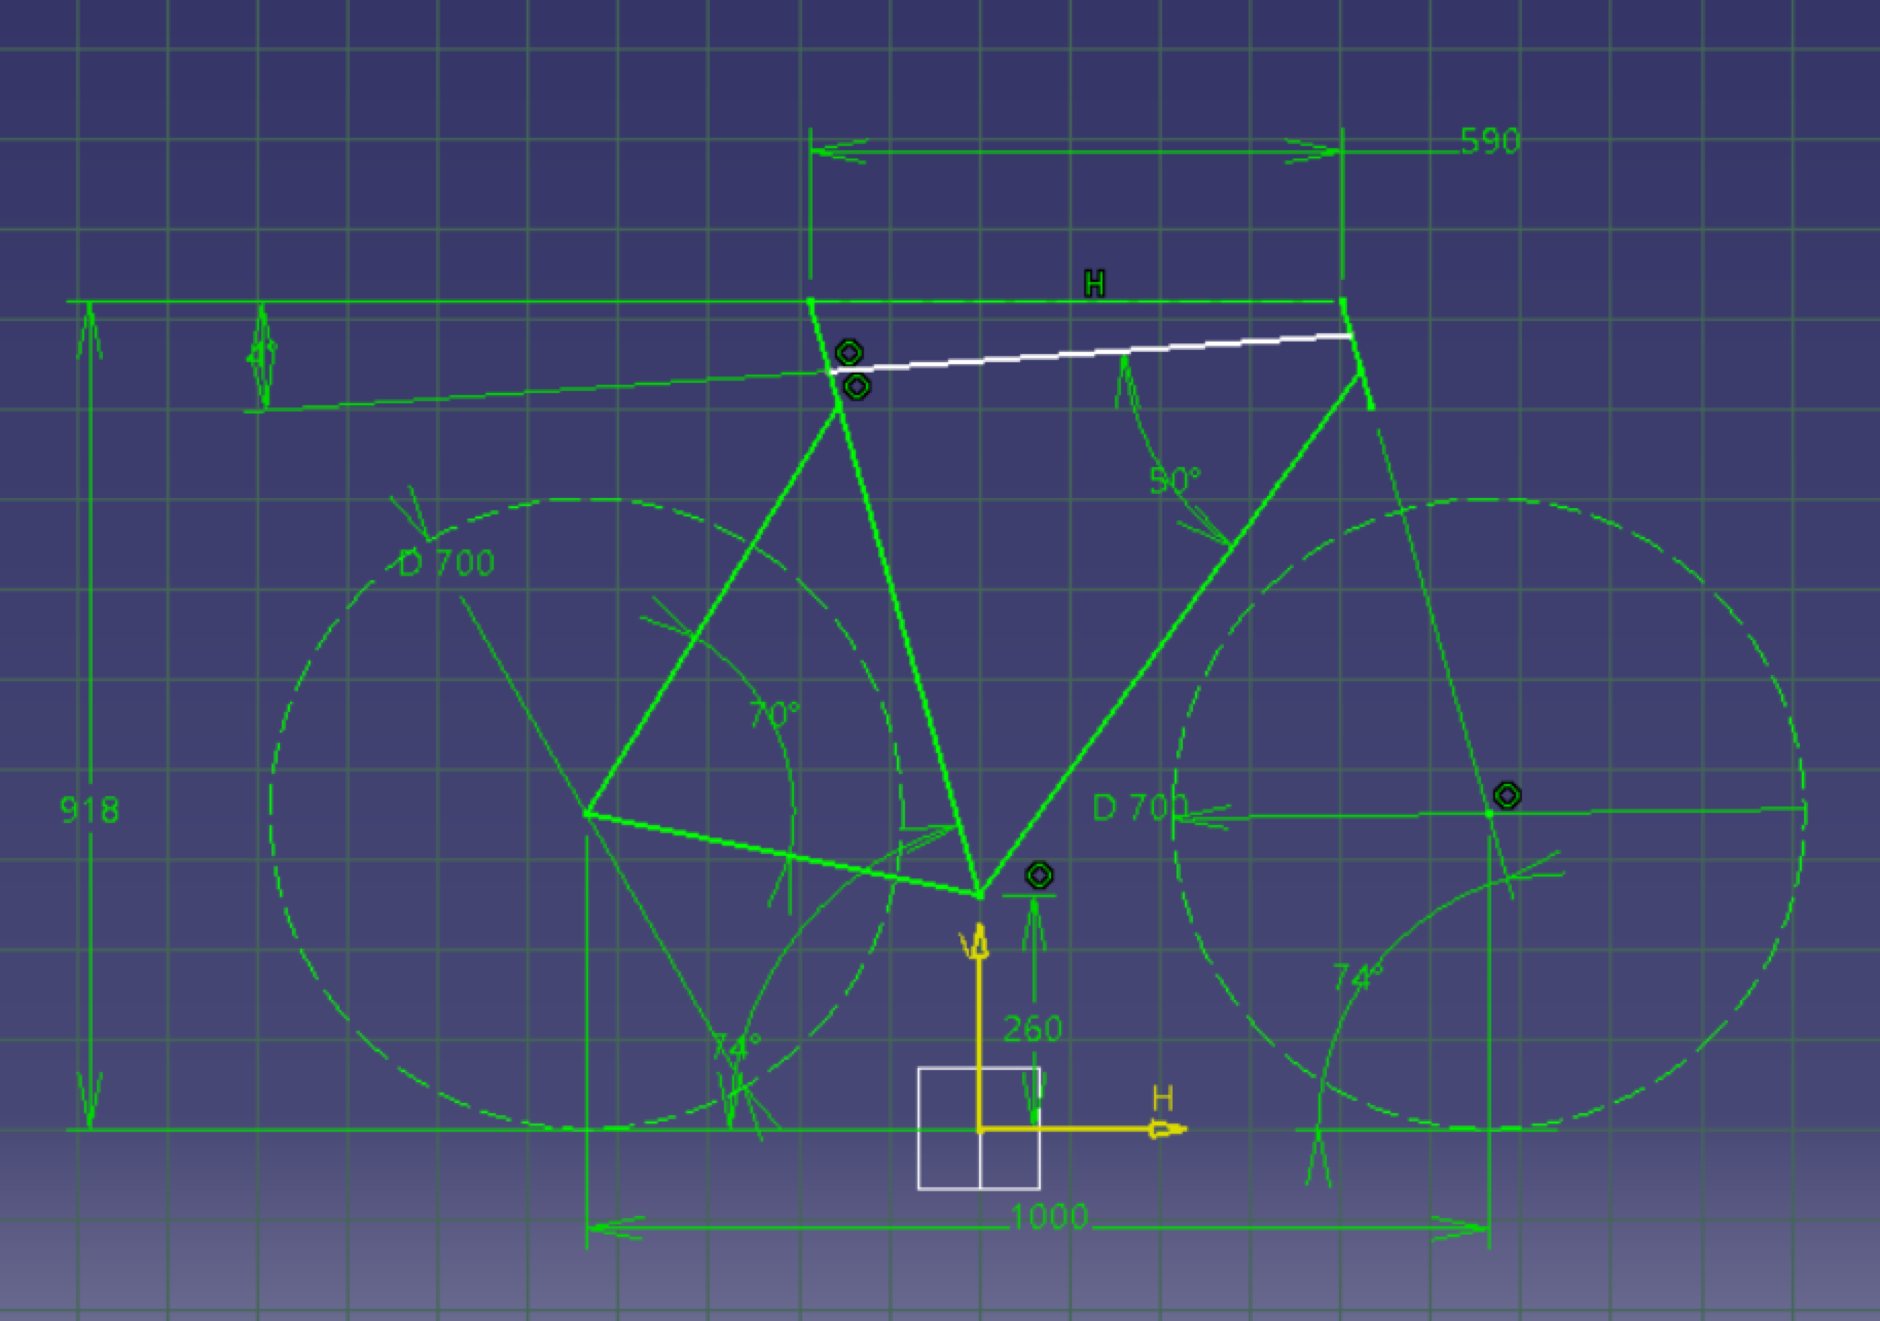
\includegraphics[scale=0.80]{dimensoes.png}
	\caption{Dimensões}
	\label{img:dimensoes}
	\end{figure}

\newpage

	\subsection{Estabilidade}
	O centro de massa da bicicleta sem os componentes se concentrou em 0,6m no eixo x e 0,5m no eixo y, as forças normais nos pneus traseiros e dianteiros foram de,respectivamente: 24,525N e 73,575N, enquanto as forças de fricção(atrito)  nos pneus traseiros e dianteiros de, respectivamente: 14,96N e 44,88N. As figuras \ref{img:esq_forca_sem_frenagem}, \ref{img:esq_forca_com_frenagem_suave} e \ref{img:esq_forca_com_frenagem_brusca} apresentam três esquemáticos demonstrando a aplicação da força sobre a bicicleta em três momentos distintos.

\graphicspath{{figuras/}}
\begin{figure}[h!]
\centering
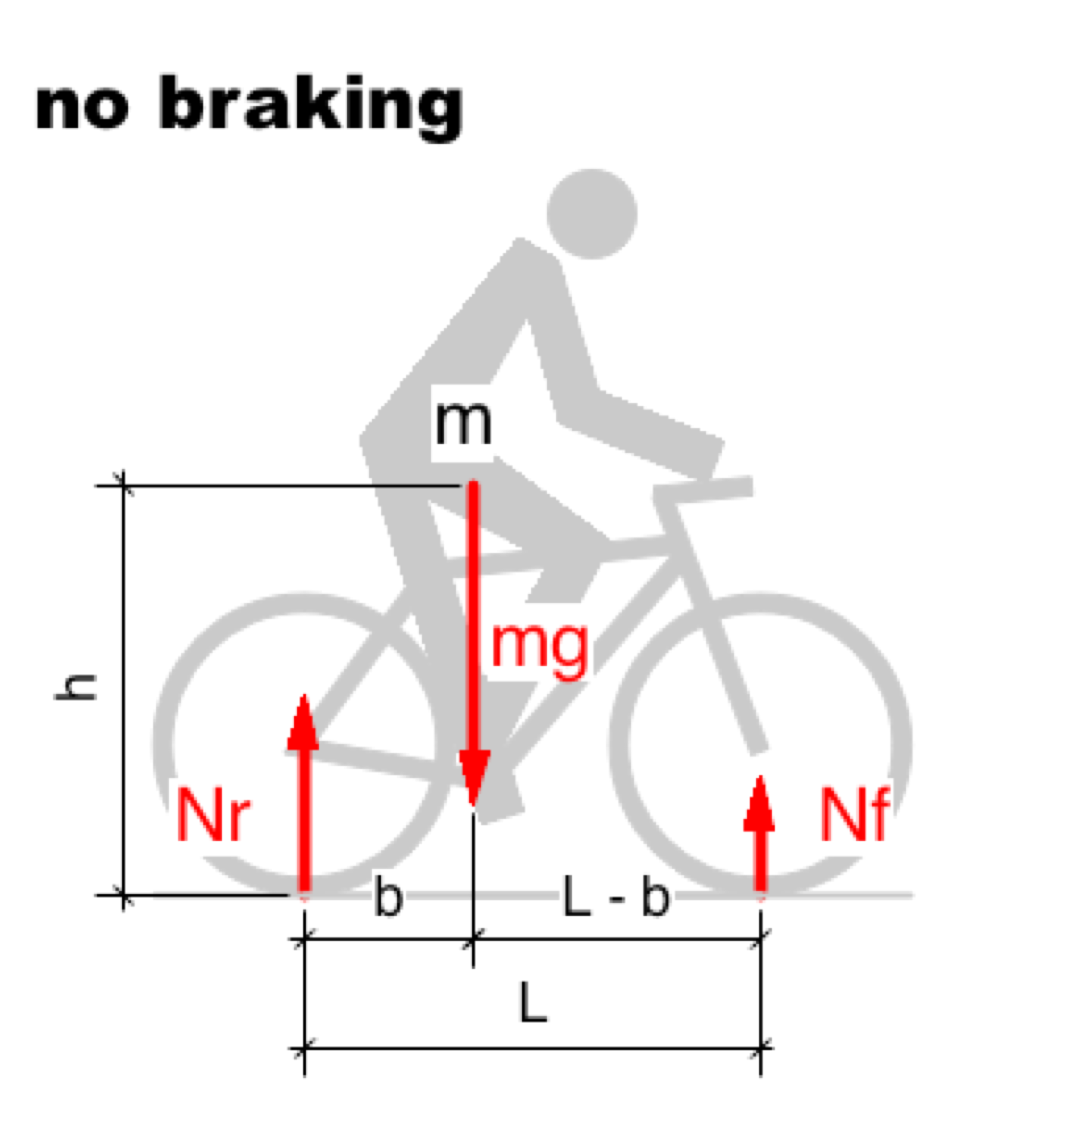
\includegraphics[scale=0.80]{esq_forca_sem_frenagem.png}
\caption{Esquemático de força sem frenagem}
\label{img:esq_forca_sem_frenagem}
\end{figure}

\graphicspath{{figuras/}}
\begin{figure}[h!]
\centering
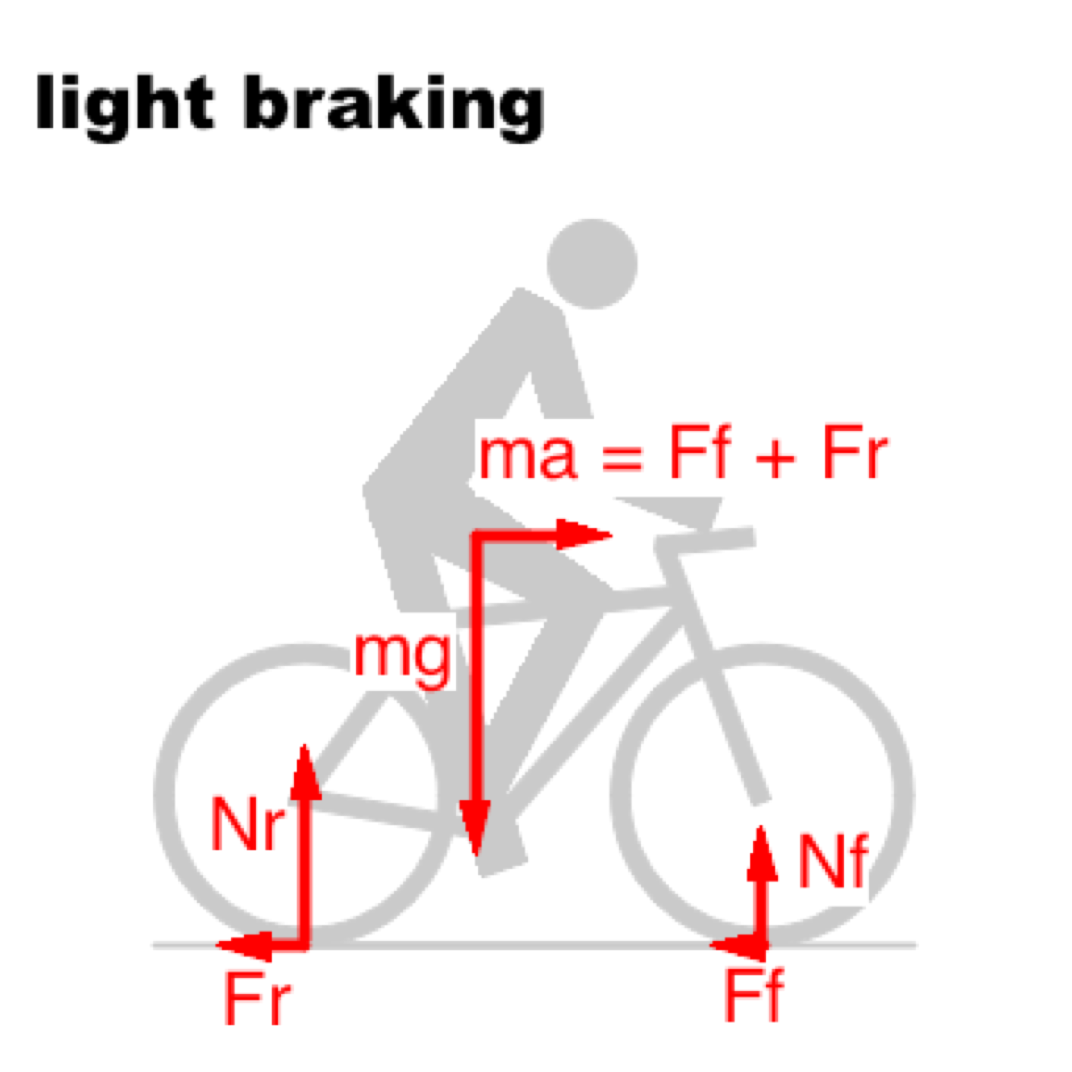
\includegraphics[scale=0.80]{esq_forca_com_frenagem_suave.png}
\caption{Esquemático de força com frenagem suave}
\label{img:esq_forca_com_frenagem_suave}
\end{figure}

\graphicspath{{figuras/}}
\begin{figure}[h!]
\centering
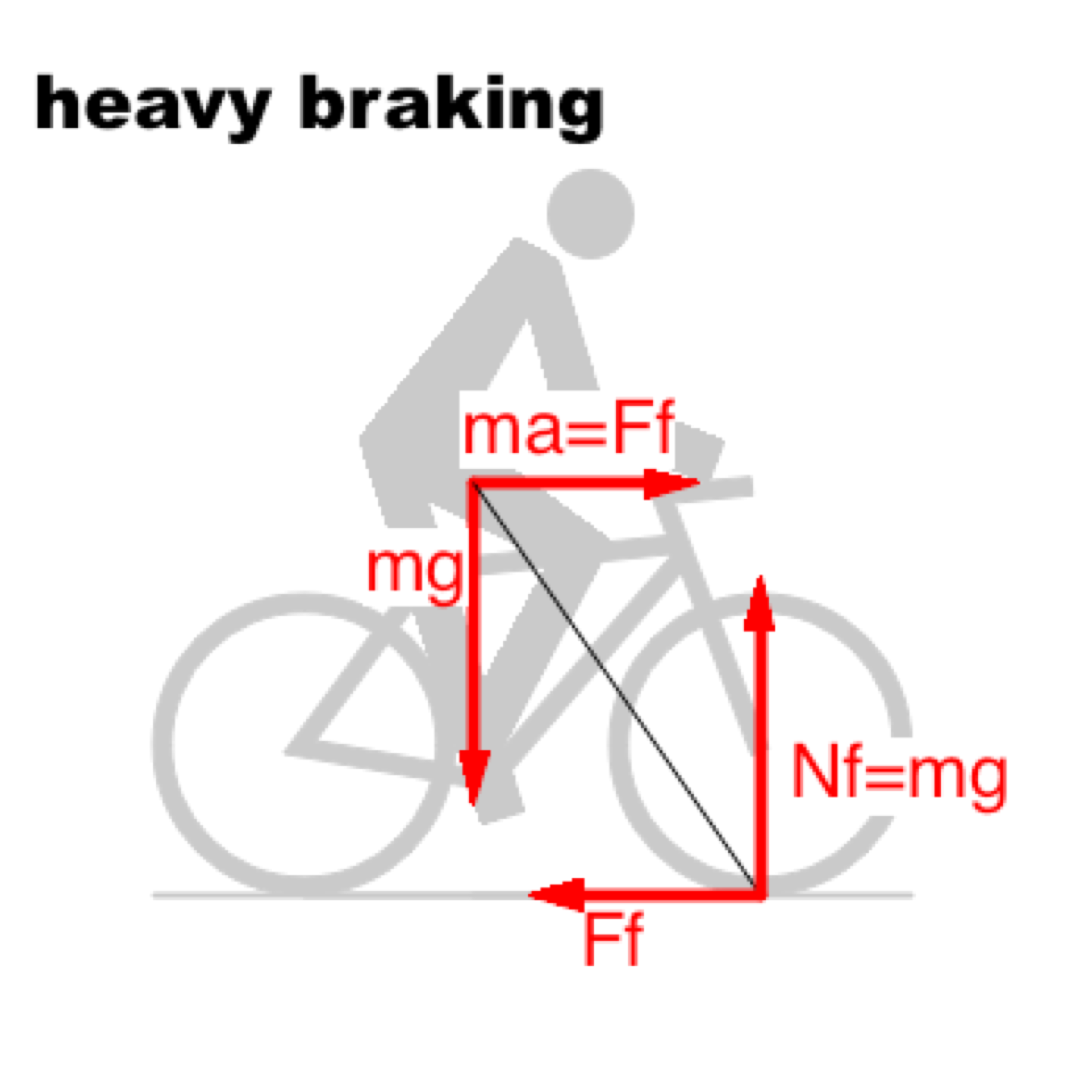
\includegraphics[scale=0.80]{esq_forca_com_frenagem_brusca.png}
\caption{Esquemático de forca com frenagem brusca}
\label{img:esq_forca_com_frenagem_brusca}
\end{figure}

\newpage

	\subsection{Análises}
	Foram feitas algumas análises em um quadro de 17 com ajuda dos softwares CATIA v5 e Ansys R17.0 no intuito de levantar questões sobre requisitos e melhorias que deverão estar presentes na estrutura.
	
	\subsection{Estática}
	As figuras \ref{img:deformacao_total}, \ref{img:equivalente_de_von_mises}, \ref{img:modo_de_vibracao}, \ref{img:modo_de_vibracao2}, \ref{img:modo_de_vibracao3}, \ref{img:modo_de_vibracao4}, \ref{img:modo_de_vibracao5} e \ref{img:modo_de_vibracao 6} apresentam alguns graus de deformação à qual a bicicleta pode ser submetida. 	
	
\graphicspath{{figuras/}}
	\begin{figure}[h!]
	\centering
	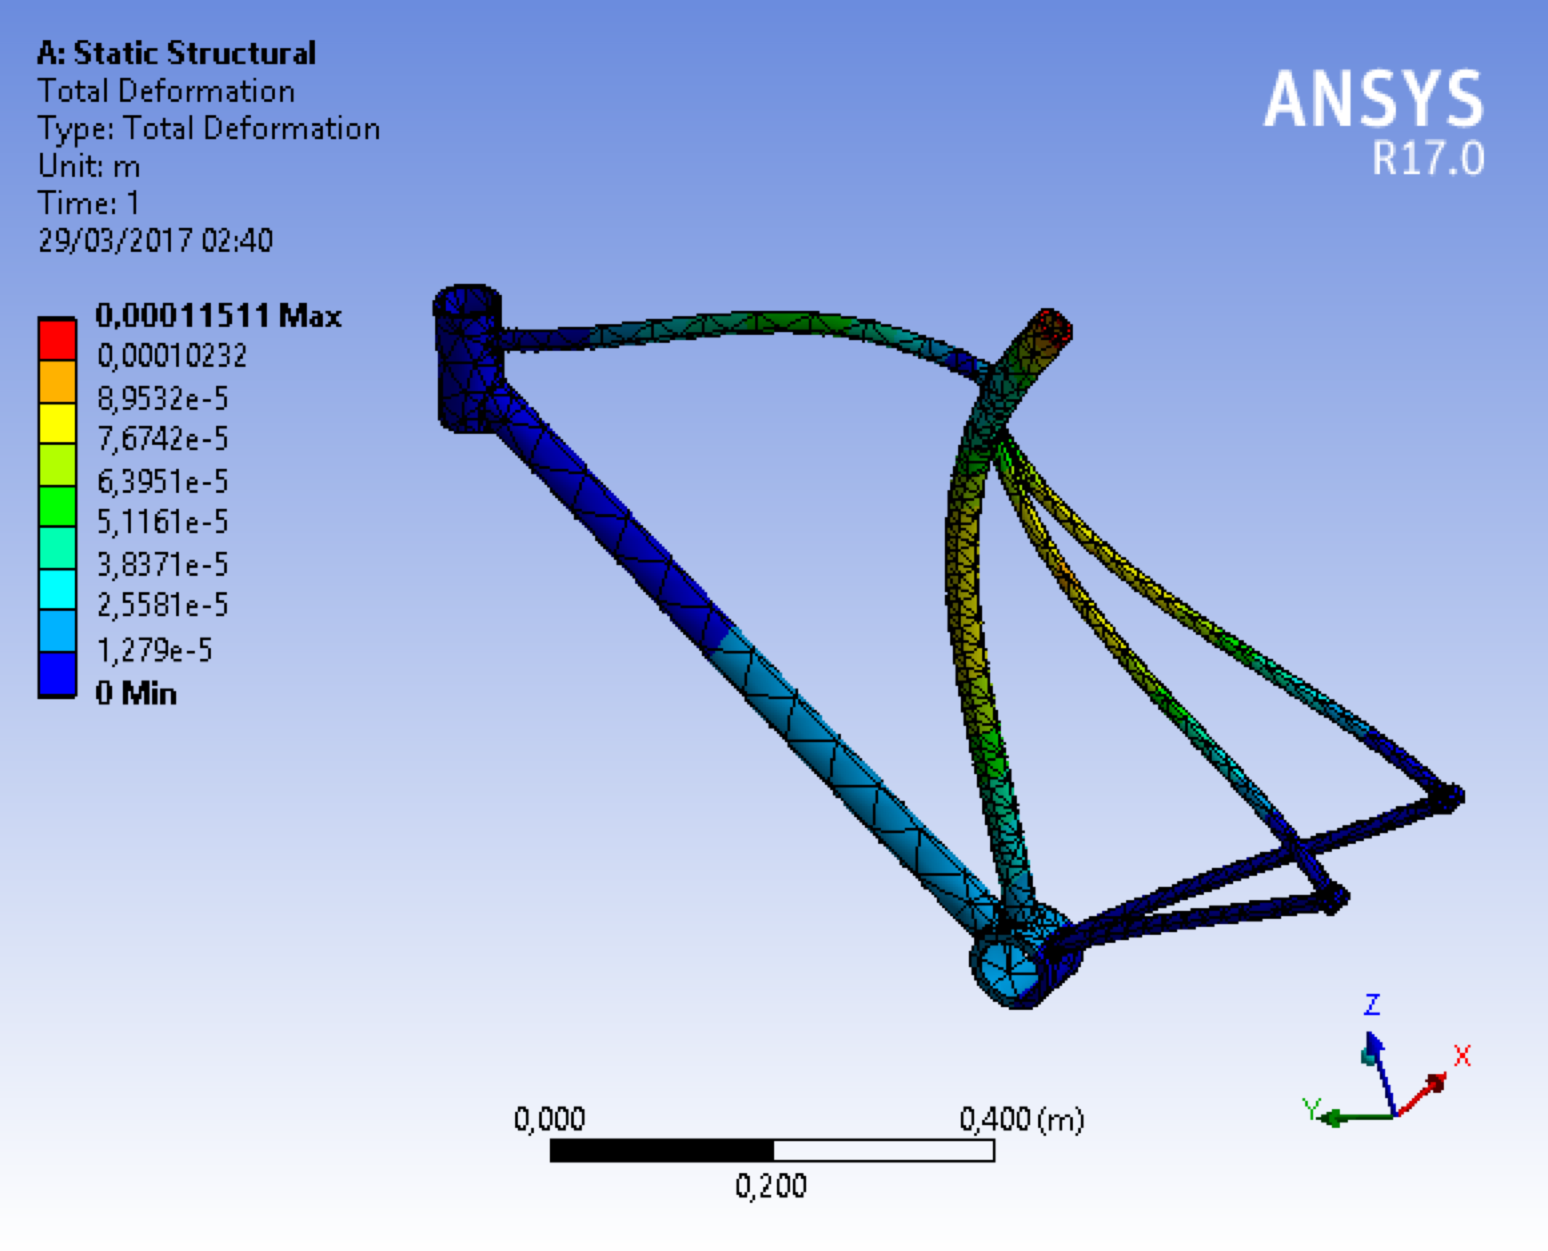
\includegraphics[width=0.7\textwidth]{deformacao_total.png}
	\caption{Deformacao total}
	\label{img:deformacao_total}
	\end{figure}	
	
\graphicspath{{figuras/}}
	\begin{figure}[h!]
	\centering
	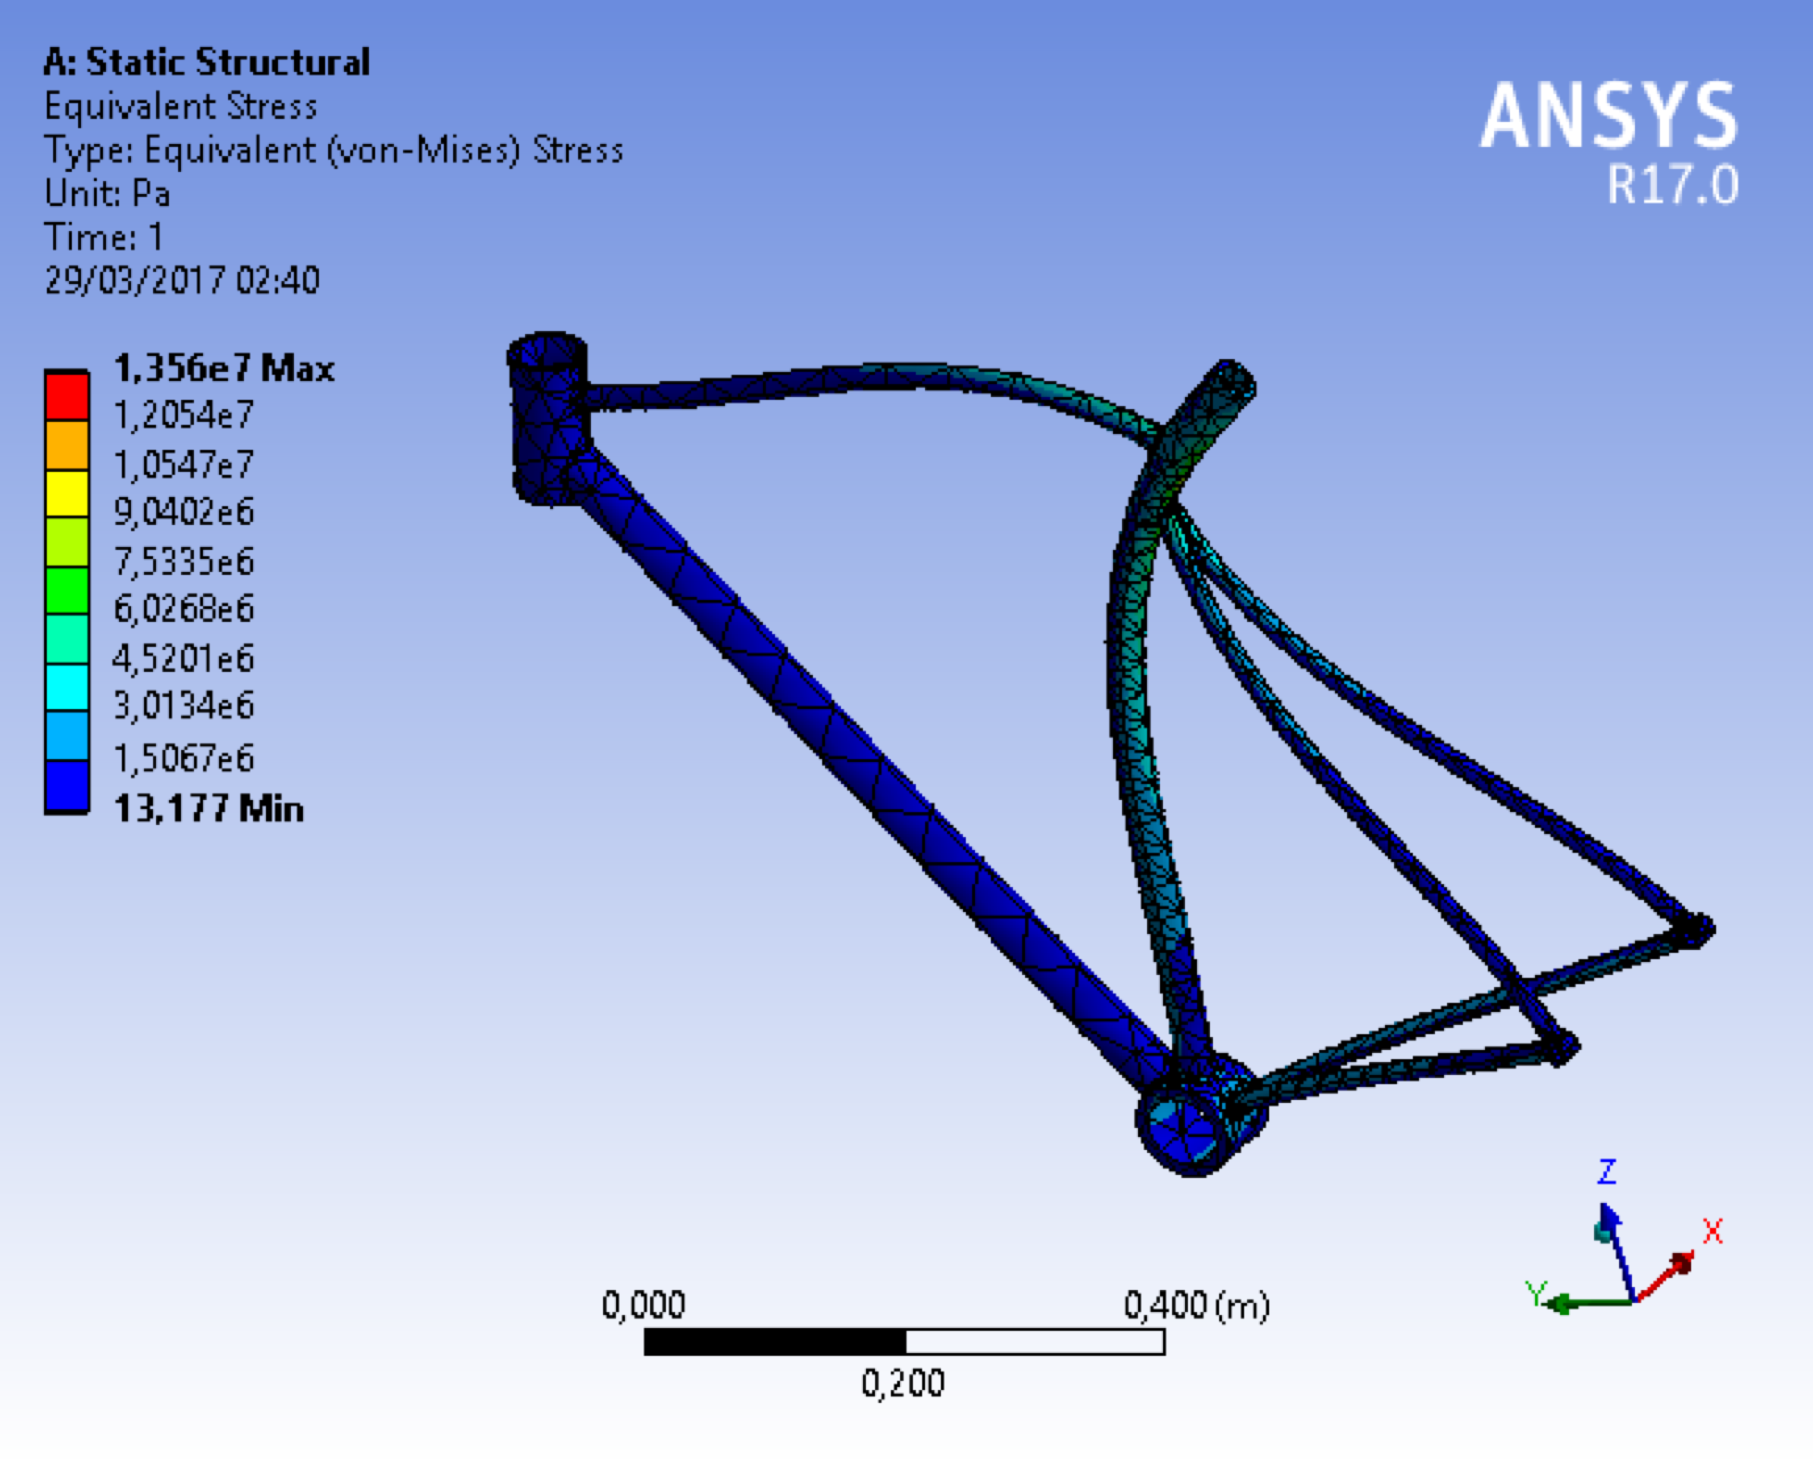
\includegraphics[width=0.7\textwidth]{equivalente_de_von_mises.png}
	\caption{Equivalente de von-Mises}
	\label{img:equivalente_de_von_mises}
	\end{figure}	
	
\graphicspath{{figuras/}}
	\begin{figure}[h!]
	\centering
	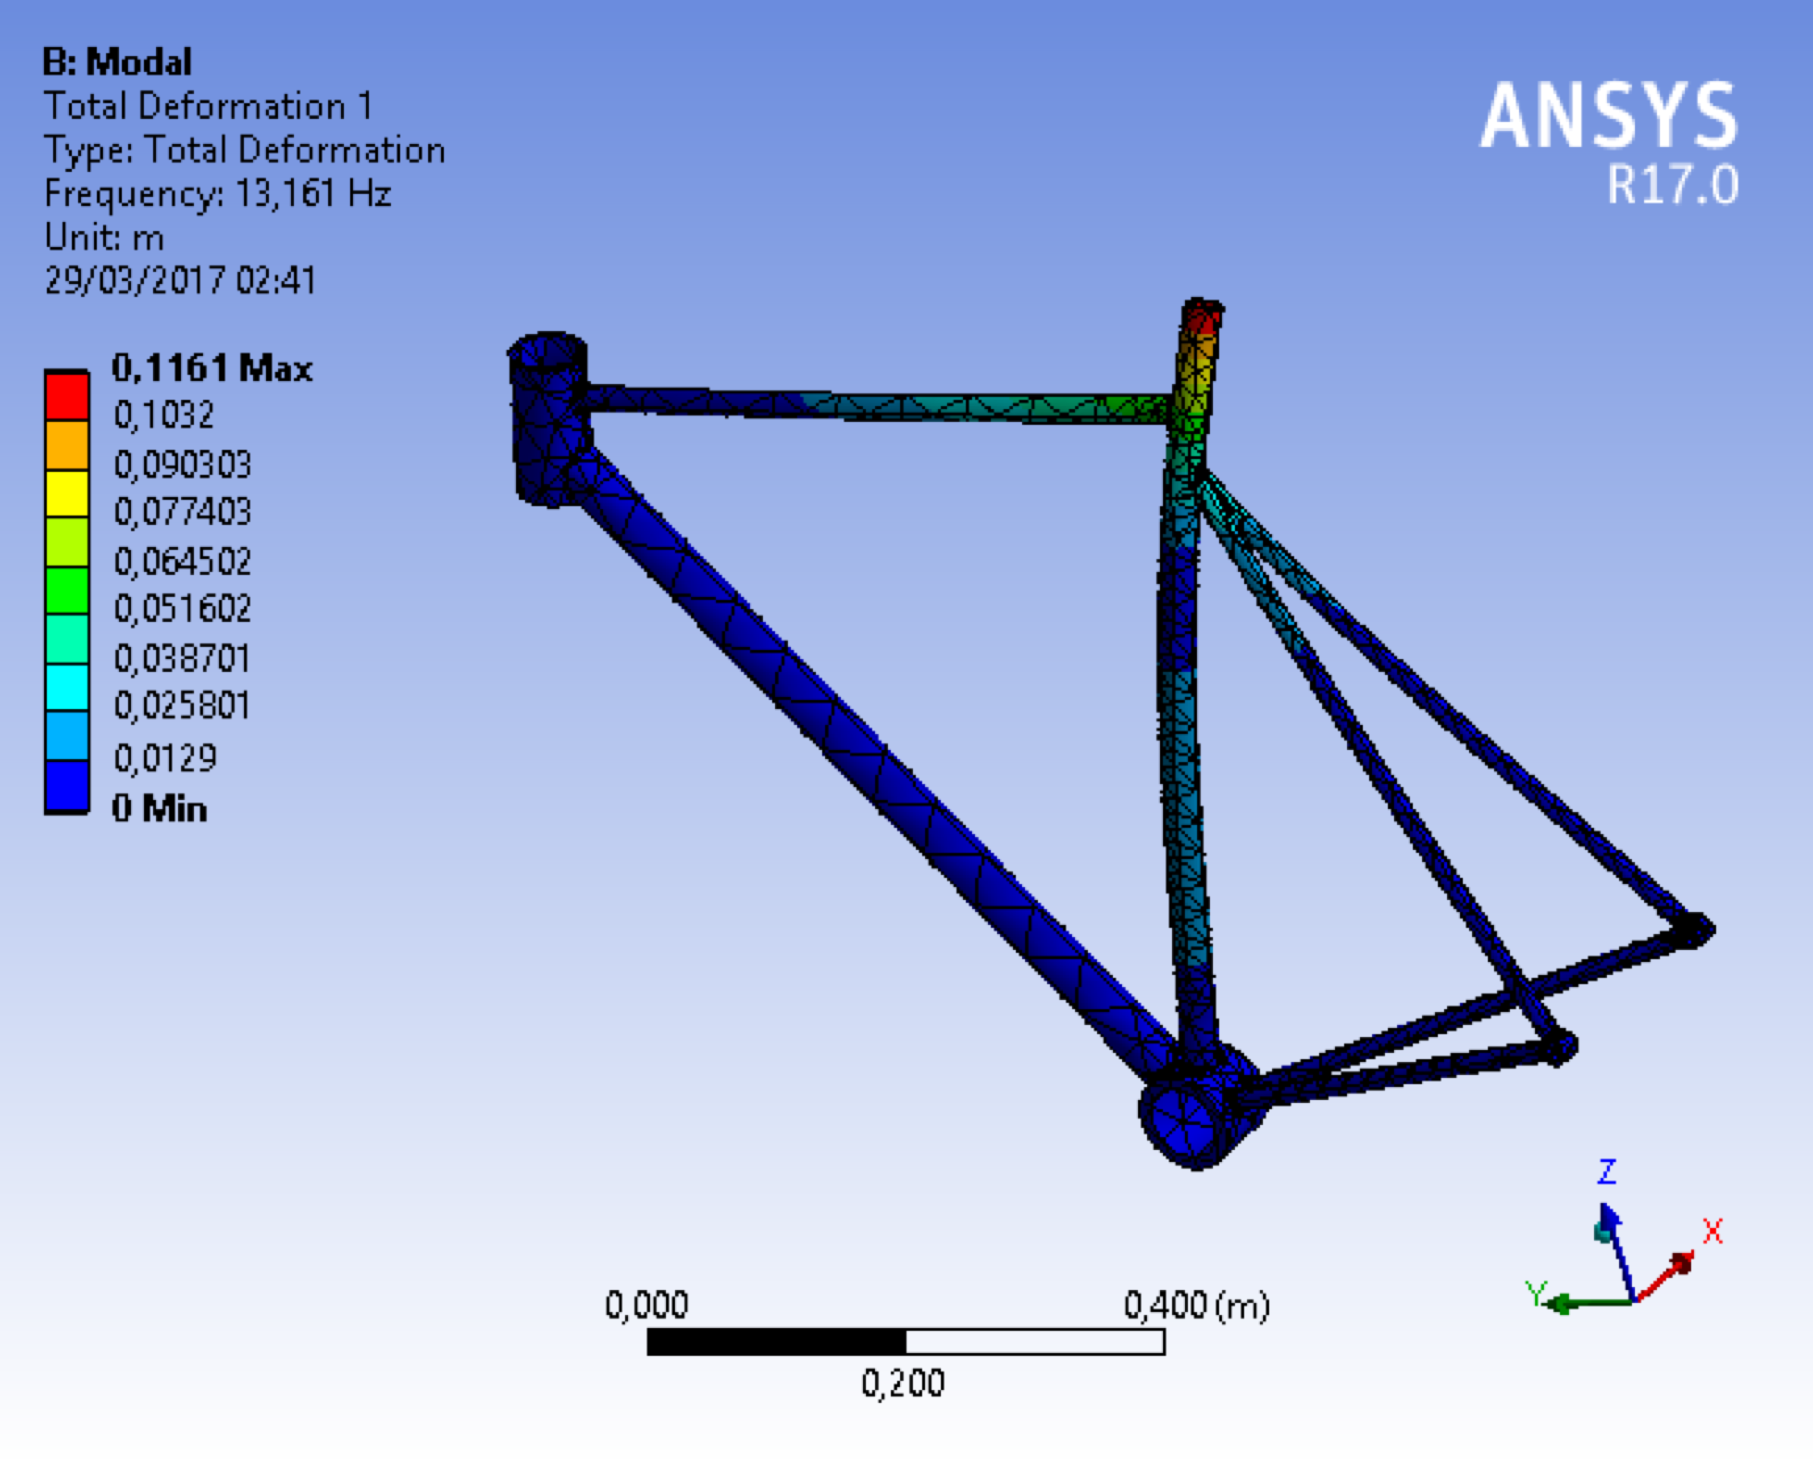
\includegraphics[width=0.7\textwidth]{modo_de_vibracao.png}
	\caption{Modo de vibração 1}
	\label{img:modo_de_vibracao}
	\end{figure}	
	
\graphicspath{{figuras/}}
	\begin{figure}[h!]
	\centering
	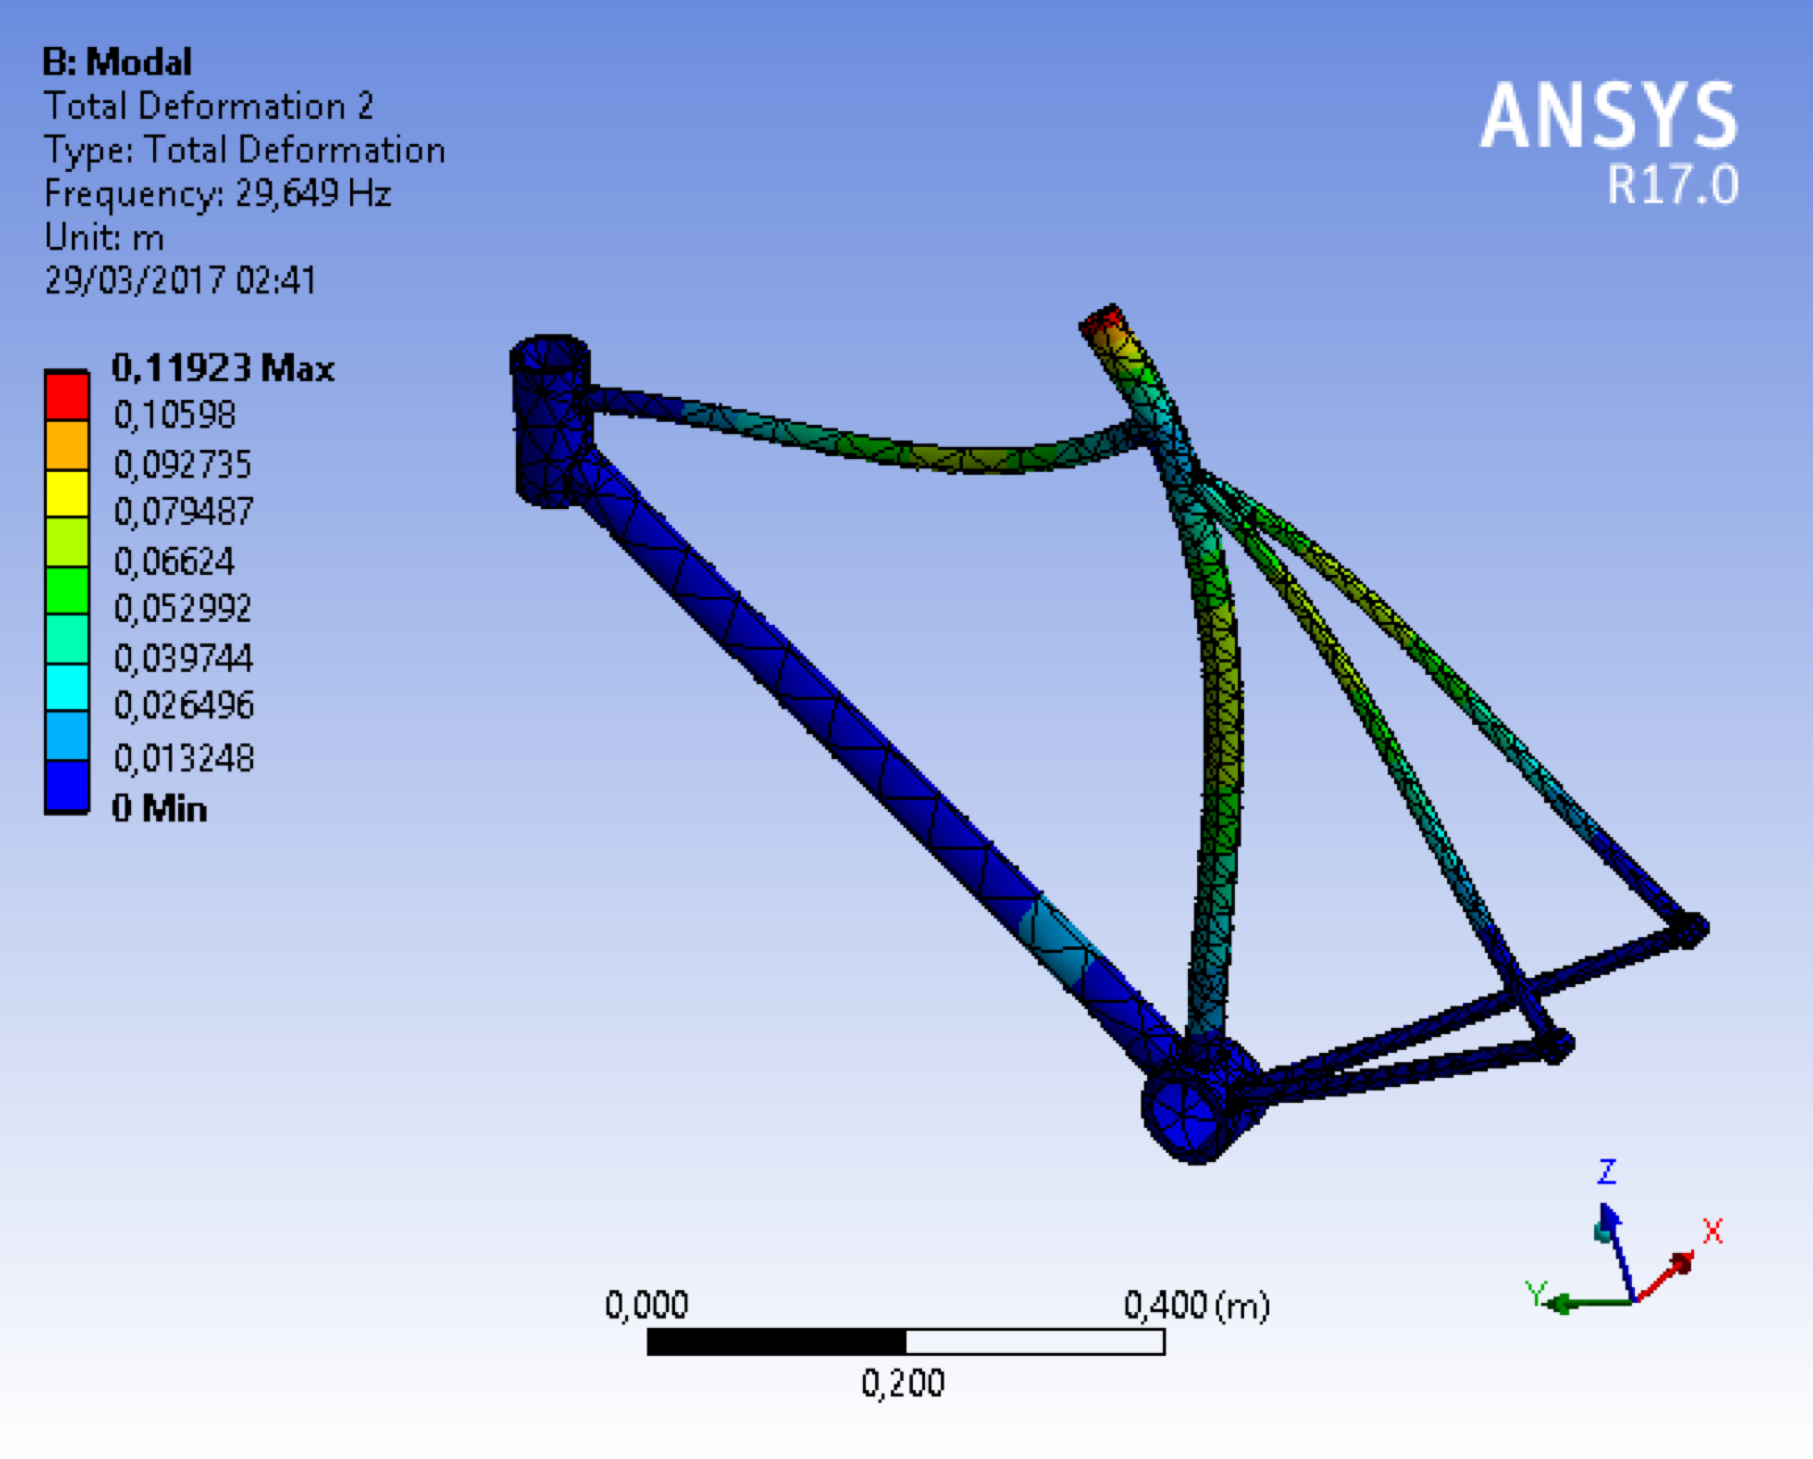
\includegraphics[width=0.7\textwidth]{modo_de_vibracao_2.png}
	\caption{Modo de vibracao 2}
	\label{img:modo_de_vibracao2}
	\end{figure}	
	
\graphicspath{{figuras/}}
	\begin{figure}[h!]
	\centering
	\includegraphics[width=0.7\textwidth]{modo_de_vibracao_3.png}
	\caption{Modo de vibração 3}
	\label{img:modo_de_vibracao3}
	\end{figure}	
	
\graphicspath{{figuras/}}
	\begin{figure}[h!]
	\centering
	\includegraphics[width=0.7\textwidth]{modo_de_vibracao_4.png}
	\caption{Modo de vibração 4}
	\label{img:modo_de_vibracao4}
	\end{figure}	
	
\graphicspath{{figuras/}}
	\begin{figure}[h!]
	\centering
	\includegraphics[width=0.7\textwidth]{modo_de_vibracao_5.png}
	\caption{Modo de vibração 5}
	\label{img:modo_de_vibracao5}
	\end{figure}	

\graphicspath{{figuras/}}
	\begin{figure}[h!]
	\centering
	\includegraphics[width=0.7\textwidth]{modo_de_vibracao_6.png}
	\caption{Modo de vibração 6}
	\label{img:modo_de_vibracao 6}
	\end{figure}	

\clearpage

	
	
	
	\subsection{Desafios Técnicos}
	Desafio: Definir uma geometria que comporte todo o sistema sem afetar a ergonomia do ciclista, e que seja capaz de suportar todas as solicitações mecânicas
Alternativa de solução: Alterar a geometria e/ou alterar o material da estrutura.

Desafio: impossibilidade de fabricação do quadro  por escassez de recursos, tempo ou incapacidade técnica.

Alternativa de solução: adquirir um quadro comum no comércio e realizar as adaptações necessárias.

	\subsection{Atualizações}
	A princípio o objetivo era a construção completa da estrutura do quadro da bicicleta, porém a fabricação de um quadro se mostrou inviável, tanto pelo custo quanto pela falta de mão de obra necessária para a criação do protótipo. Desta forma procurou-se viabilizar o projeto a partir de modificações estruturais em uma bicicleta comum. 
	Para o motor elétrico foi necessário uma roda aro 29”. Assim foi iniciada uma procura por um quadro de 29”, inicialmente procurou-se por quadros e bicicletas novas, visto que o custo era bastante elevado, foi ampliada a busca por quadros e bicicletas completas usadas. Chegou-se à conclusão de que uma bicicleta completa usada reduziria os custos, dado que não seria necessária a compra de todos os materiais que compõem a bicicleta. 
	Como no primeiro ponto de controle foi proposto que o material da bicicleta seria alumínio, mantivemos essa diretriz na busca. Encontrada a bicicleta, partimos para o projeto de quais adaptações seriam necessárias para assegurar que a estrutura suportaria todas as necessidades do projeto.
	
	A bicicleta escolhida foi uma modelo M7 da marca GTMAX já equipada com os seguintes componentes:
	\begin{itemize}
		\item Aro: Aero 29 Alumínio Vnezi Vzan
		\item Cubo dianteiro/traseiro: 36F em alumínio com blocagem preto
		\item Raio: 290 x 2,0 zincado
		\item Câmara de Ar: 29 importado
		\item Pneu: 29 x 1,95 de cravo preto
		\item Selim: MTB preto Cairu
		\item Canote: Selim em alumínio com blocagem preta
		\item Pedal:9/16 Mtb em alumínio
		\item Abraçadeira de alumínio com blocagem preta
		\item Movimento central com rolamento Shunfeng
		\item Movimento de direção ahead set Neco preto
		\item Pedivela com engrenagem tripla de alumínio preto
		\item Alavanca Eze Fire EF40 7 velocidade Shimano
		\item Suporte de guidão alumínio ahead set preto Unicicle
		\item Guidão curvo expandido de aço preto importado
		\item Roda livre 7 velocidades Index Skyrano
		\item Câmbio dianteiro/traseiro Tz 31 sem gancheira Shimano
		\item Corrente fina Index IG 51
		\item Garfo de suspensão: 29 Over em aço/alumínio preto Verselli
		\item Quadro de alumínio: 29" GTMAX M7 19"
		\item Freio a disco dianteiro/traseiro Sypo 21 velocidades
	\end{itemize}

	Logo após a aquisição a bicicleta foi desmontada deixando o quadro como na Figura \ref{img:quadro_original_lateral} e \ref{img:quadro_original_fundo} para facilitar a obtenção das medidas e assim tornar possível a confecção do modelo CAD no Catia V5 com a adaptação eleita.
		
	\graphicspath{{figuras/}}
	\begin{figure}[h!]
		\centering
		\includegraphics[width=0.5\textwidth]{quadro_original_lateral.jpg}
		\caption{Quadro original (vista lateral)}
		\label{img:quadro_original_lateral}
	\end{figure}

	\graphicspath{{figuras/}}
	\begin{figure}[h!]
		\centering
		\includegraphics[width=0.3\textwidth]{quadro_original_fundo.jpg}
		\caption{Detalhe do fundo do quadro original}
		\label{img:quadro_original_fundo}
	\end{figure}
	
	Nas Figuras \ref{img:inter_render} e \ref{img:inter_cotas} é possível visualizar  o resultado da modelagem e algumas cotas importantes para o desenvolvimento do projeto.
	
	\graphicspath{{figuras/}}
	\begin{figure}[h!]
		\centering
		\includegraphics[scale=0.035]{inter_render_2.jpg}
		\includegraphics[scale=0.035]{inter_render_1.jpg}
		\caption{Quadro renderizado no Catia V5}
		\label{img:inter_render}
	\end{figure}
	
	%\graphicspath{{figuras/}}
	%\begin{figure}[h!]
	%	\centering
	%	\includegraphics[scale=0.05]{inter_render_2.jpg}
	%	\caption{Detalhe do fundo do quadro original}
	%	\label{img:inter_render}
	%\end{figure}

	%\graphicspath{{figuras/}}
	%\begin{figure}[h!]
	%	\centering
	%	\includegraphics[scale=0.05]{inter_render_1.jpg}
	%	\caption{Detalhe do fundo do quadro original}
	%	\label{img:inter_render_1}
	%\end{figure}
	
	\graphicspath{{figuras/}}
	\begin{figure}[h!]
		\centering
		\includegraphics[width=0.6\textwidth]{inter_cotas.jpg}
		\caption{Detalhe do fundo do quadro original}
		\label{img:inter_cotas}
	\end{figure}
	
	\subsection{Análises}
	
	Com base no público alvo e no dimensionamento levantado pelos demais subsistemas, arbitrou-se a força peso do ciclista e do conjunto dispositivos que serão postos sobre a adaptação como 900 e 120, respectivamente. A aplicação delas estão representadas nas Figuras \ref{img:inter_F120} e \ref{img:inter_F900}. 
	
	
	\graphicspath{{figuras/}}
	\begin{figure}[h!]
		\centering
		\includegraphics[width=0.7\textwidth]{inter_F120.png}
		\caption{Força aplicada na adaptação}
		\label{img:inter_F120}
	\end{figure}
	
	\graphicspath{{figuras/}}
	\begin{figure}[h!]
		\centering
		\includegraphics[width=0.7\textwidth]{inter_F900.png}
		\caption{Força peso do ciclista}
		\label{img:inter_F900}
	\end{figure}
	
	Como esses dados foi feito a análise estática no Ansys, nas Figuras \ref{img:inter_deformacao_total}, \ref{img:inter_von-Mises}, \ref{img:inter_fator_de_seguranca} e \ref{img:inter_fadiga} representam, respectivamente, os gradientes de: deformação, equivalente de von-Mises, fator de segurança e fadiga.
	
	\graphicspath{{figuras/}}
	\begin{figure}[h!]
		\centering
		\includegraphics[width=0.7\textwidth]{inter_deformacao_total.png}
		\caption{Deformação total}
		\label{img:inter_deformacao_total}
	\end{figure}
	
	\graphicspath{{figuras/}}
	\begin{figure}[h!]
		\centering
		\includegraphics[width=0.7\textwidth]{inter_von-Mises.png}
		\caption{Equivalente de von-Mises}
		\label{img:inter_von-Mises}
	\end{figure}
	
	\graphicspath{{figuras/}}
	\begin{figure}[h!]
		\centering
		\includegraphics[width=0.7\textwidth]{inter_fator_de_seguranca.png}
		\caption{Fator de segurança}
		\label{img:inter_fator_de_seguranca}
	\end{figure}

	\graphicspath{{figuras/}}
	\begin{figure}[h!]
		\centering
		\includegraphics[width=0.7\textwidth]{inter_fadiga.png}
		\caption{Fadiga}
		\label{img:inter_fadiga}
	\end{figure}
	Os resultados mostram que a estrutura proposta atende a todos os requisitos do estudados no âmbito estático.
	
	\subsection{Construção}
	
	Com a validação numérica do modelo, prosseguiu-se para a etapa de confecção do mesmo onde primeiramente foram feitos cortes no quadro original para retirar o tubo inferior como pode ser visto nas Figuras \ref{img:quadro_cerrado_lateral}, \ref{img:quadro_cerrado_1} e \ref{img:quadro_cerrado_2}.
	
		
	\graphicspath{{figuras/}}
	\begin{figure}[h!]
		\centering
		\includegraphics[width=0.7\textwidth]{quadro_cerrado_lateral.jpg}
		\caption{Quadro cerrado e lixado (vista lateral)}
		\label{img:quadro_cerrado_lateral}
	\end{figure}
	
	\graphicspath{{figuras/}}
	\begin{figure}[h!]
		\centering
		\includegraphics[width=0.3\textwidth]{quadro_cerrado_1.jpg}
		\caption{Quadro cerrado e lixado (detalhe 1)}
		\label{img:quadro_cerrado_1}
	\end{figure}
	
	\graphicspath{{figuras/}}
	\begin{figure}[h!]
		\centering
		\includegraphics[width=0.3\textwidth]{quadro_cerrado_2.jpg}
		\caption{Quadro cerrado e lixado (detalhe 2)}
		\label{img:quadro_cerrado_2}
	\end{figure}
	
	Para a construção da parte inferior do quadro foram utilizados tubos de alumínio 6060 com 1” de diâmetro e 1/8” de espessura. Primeiramente foram feitas as dobras dos tubos e verificados os ângulos através da impressão em papel A1 do drafting da peça, o desenho técnico utilizado no gabarito pode ser visto no Apêndice \ref*{gabarito}. Depois de feitas as dobras seguiu-se para o corte das quatro peças centrais. Com as quatro peças centrais prontas e as outras duas dobradas, prosseguiu-se para o processo de solda da peça completa e finalmente para a implementação da peça ao quadro.
	
	
	\graphicspath{{figuras/}}	
	\begin{figure}[h!]
		\centering
		\includegraphics[height=\textwidth,angle=-90]{gabarito.jpg}
		\includegraphics[width=\textwidth]{gabarito_adap.jpg}
		\caption{Gabarito e adaptação}
		\label{img:gabarito_adap}
	\end{figure}

	Durante o processo de dobra dos tubos de alumínio, foi notado a impossibilidade de conseguir fazer uma dobra igual a pré determinada pelo drafting, por falta de equipamento para tal, desta forma adaptamos para com que a dobra feita fosse satisfatória.
	
	Todo o processo de construção foi auxiliado pelo prestador de serviços especializado em solda em alumínio, Mateus Silva de Almeida, desde o corte do quadro à solda, sendo que esta última etapa foi inteiramente realizada por ele. A adaptação fez-se necessária para suportar todos os componentes eletroeletrônicos que a bicicleta elétrica transportará.
	
	A Figura \ref{img:quadro_adap_1} mostra o produto final oriundo da adaptação do quadro.

	\graphicspath{{figuras/}}	
	\begin{figure}[h!]
		\centering
		\includegraphics[width=0.7\textwidth]{quadro_adap_1.jpg}
		\caption{Quadro com a adaptação}
		\label{img:quadro_adap_1}
	\end{figure}
	
	Para viabilizar o projeto já descrito acima foram necessários os gastos listados na Tabela \ref*{custo_dos_materiais_da_estrutura} a seguir:
	
	
	\newcolumntype{M}[1]{>{\centering\arraybackslash}m{#1}}
	\begin{table}[!htb]
		\centering
		\caption{Custo dos Materiais da Estrutura}
		\begin{tabular}{|M{6cm} | M{3,5cm} |}
			\hline
			\textbf{MATERIAL} & \textbf{Preço(R\$)} \\ \hline
			Bicicleta M7 GTMAX usada & 700,00 \\
			\hline
			Solda de adaptação do quadro & 250,00\\
			\hline
			Quatro metros de tubos de alumínio 6060, 1” de diâmetro, 1/8” de parede. & 100,00\\
			\hline
			Impressão em Folha A1 & 6,00\\
			\hline
			Desmontagem da corrente & 15,00\\
			\hline
			
		\end{tabular}
		\label{custo_dos_materiais_da_estrutura}
	\end{table}
	
\clearpage


  \section{Normas}
  Para garantir a integridade e segurança do projeto e dos futuros usuários do produto, deve-se atentar a determinadas normas técnicas, que garantem a funcionalidade do projeto. Essas normas ajudam a definir diversas características de um produto, visando uma padronização que auxilia na solução de futuros problemas, assegurando a qualidade e eficiência desejada. No Brasil, a Agência Brasileira de Normas Técnicas (ABNT) é o órgão responsável pela elaboração das Normas Técnicas Brasileiras (NBR), que servem como instrumento na avaliação de conformidades e certificação de diversas áreas e produtos, garantindo a devida credibilidade. Para o caso da Smart Bike, alguns itens importantes podem ser destacados diante da NBR NM 213, que é uma norma específica voltada para Princípios de Projeto e Segurança de Equipamentos Eletromecânicos.
  

\newcolumntype{M}[1]{>{\centering\arraybackslash}m{#1}}
\begin{table}[!htb]
	\centering
	\caption{Tabela de Normas}
	\begin{tabular}{|M{2,5cm} | M{4,5cm} | M{9cm}|}
		\hline
		\textbf{ITEM AVALIADO} & \textbf{MEDIDA NORMATIVA} & \textbf{O QUE SERÁ FEITO?} \\ \hline
		Arestas vivas, ângulos vivos, peças salientes, etc. & Prevenir, durante o uso da bicicleta, o acesso do usuário aos pontos de risco. & Será feita uma análise do projeto estrutural para proteger, cercar e alinhar qualquer design estrutural que fornecer perigo físico ao usuário. \\
		\hline
		Formas e posição de componentes & Garantir que os componentes sejam posicionados da forma mais adequada ao projeto e a segurança do usuário. & Os componentes serão posicionados de maneira otimizada com sua função, evitando gambiarras e grandes conexões. Os motores e baterias não serão acessíveis ao usuário enquanto o mesmo estiver pedalando. \\
		\hline
		Ergonomia & Reduzir as tensões nervosas e o esforço físico do usuário. & A bicicleta terá, no seu banco e guidon, regulagem de altura para garantir ao usuário o maior conforto possível. \\
		\hline
		Sistema de comando & Garantir o acesso do usuário à informações gerais do sistema, assim como, sua intervenção. & Através de um display o usuário será capaz de saber as principais informações de operação da bicicleta, como nível de carga da bateria e velocidade. O usuário poderá cessar o funcionamento do motor através de um simples botão de partida. \\
		\hline
		Perigo Elétrico & Proteções contra choques elétricos, curtos circuitos e sobrecargas. & Haverá uma blindagem no circuito elétrico para proteger o usuário do acesso as conexões elétricas que alimentam a bateria e o motor. \\
		\hline
		Estrutura & Robustez & A estrutura será projetada para suportar determinadas cargas de peso e fadiga que serão submetidas à bicicleta. \\
		\hline
		Exigências gerais, avisos, instruções. & Deve existir clareza nas informações de operação. & O acionamento do motor será feito por uma chave de partida simples que, automaticamente, irá ligar todo o sistema de controle, tornando acessível a utilização do usuário ao sistema. \\
		\hline
		Documento de acompanhamento & Manual de instrução & Será elaborado um documento abordando os itens de segurança, utilização, armazenamento, situações de emergência, etc. \\
		\hline
		Medidas adicionais & Medidas previstas para situações de emergência. & Será elaborado um dispositivo de parada de emergência técnica, trazendo a operação da bicicleta para o modo manual. \\
		\hline
		Manutenção & Considerar fatores que facilitem a manutenabilidade do sistema. & A estrutura será montada de maneira que torne fácil o acesso as partes e sistemas internos. \\
		\hline
	\end{tabular}
	\label{tabela_normas}
\end{table}

\begin{comment}
	\begin{table}[!htbp]
	\centering
	\caption{Tabela de Normas}
	\label{tabela_normas1}
	\begin{tabular}{|lll|}
	\hline
	\multicolumn{1}{|l|}{\textbf{ITEM AVALIADO}}                                                   & \multicolumn{1}{l|}{\textbf{MEDIDA NORMATIVA}}                                                                                                             & \textbf{O QUE SERÁ FEITO?}                                                                                                                                                                                                                                                                        \\ \hline
	\begin{tabular}[c]{@{}l@{}}Arestas vivas, ângulos vivos, \\ peças salientes, etc.\end{tabular} & \begin{tabular}[c]{@{}l@{}}Prevenir, durante o uso \\ da bicicleta, o acesso do \\ usuário aos pontos de risco\end{tabular}                                & \begin{tabular}[c]{@{}l@{}}Será feita uma análise do projeto estrutural \\ para proteger, cercar e alinhar qualquer design \\ estrutural que fornecer perigo físico ao usuário\end{tabular}                                                                                                       \\ \hline
	\begin{tabular}[c]{@{}l@{}}Formas e posição de \\ componentes\end{tabular}                     & \begin{tabular}[c]{@{}l@{}}Garantir que os componentes \\ sejam posicionados da forma \\ mais adequada ao projeto e a \\ segurança do usuário\end{tabular} & \begin{tabular}[c]{@{}l@{}}Os componentes serão posicionados de \\ maneira otimizada com sua função, \\ evitando gambiarras e grandes conexões. \\ Os motores e baterias não serão acessíveis \\ ao usuário enquanto o mesmo estiver pedalando.\end{tabular}                                      \\ \hline
	Ergonomia                                                                                      & \begin{tabular}[c]{@{}l@{}}Reduzir as tensões nervosas e \\ o esforço físico do usuário.\end{tabular}                                                      & \begin{tabular}[c]{@{}l@{}}A bicicleta terá, no seu banco e guidon, regulagem \\ de altura para garantir ao usuário o maior conforto possível\end{tabular}                                                                                                                                        \\ \hline
	Sistema de comando                                                                             & \begin{tabular}[c]{@{}l@{}}Garantir o acesso do usuário à \\ informações gerais do sistema,\\ assim como, sua intervenção.\end{tabular}                    & \begin{tabular}[c]{@{}l@{}}Através de um display o usuário será capaz de saber \\ as principais informações de operação da bicicleta, \\ como nível de carga da bateria e velocidade. O usuário \\ poderá cessar o funcionamento do motor através de \\ um simples botão de partida.\end{tabular} \\ \hline
	Perigo Elétrico                                                                                & \begin{tabular}[c]{@{}l@{}}Proteções contra choques elétricos, \\ curtos circuitos e sobrecargas\end{tabular}                                              & \begin{tabular}[c]{@{}l@{}}Haverá uma blindagem no circuito elétrico para \\ proteger o usuário do acesso as conexões elétricas \\ que alimentam a bateria e o motor\end{tabular}                                                                                                                 \\ \hline
	Estrutura                                                                                      & Robustez                                                                                                                                                   & \begin{tabular}[c]{@{}l@{}}A estrutura será projetada para suportar determinadas \\ cargas de peso e fadiga que serão submetidas à bicicleta.\end{tabular}                                                                                                                                        \\ \hline
	\begin{tabular}[c]{@{}l@{}}Exigências gerais, \\ avisos, instruções\end{tabular}               & \begin{tabular}[c]{@{}l@{}}Deve existir clareza nas \\ informações de operação\end{tabular}                                                                & \begin{tabular}[c]{@{}l@{}}O acionamento do motor será feito por uma chave de \\ partida simples que, automaticamente, irá ligar todo o \\ sistema de controle, tornando acessível a utilização \\ do usuário ao sistema\end{tabular}                                                             \\ \hline
	Documento de acompanhamento                                                                    & Manual de instrução                                                                                                                                        & \begin{tabular}[c]{@{}l@{}}Será elaborado um documento abordando os itens \\ de segurança, utilização, armazenamento, situações de \\ emergência, etc.\end{tabular}                                                                                                                               \\ \hline
	Medidas adicionais                                                                             & \begin{tabular}[c]{@{}l@{}}Medidas previstas para situações \\ de emergência\end{tabular}                                                                  & \begin{tabular}[c]{@{}l@{}}Será elaborado um dispositivo de parada de emergência\\  técnica, trazendo a operação da bicicleta para o \\ modo manual.\end{tabular}                                                                                                                                 \\ \hline
	Manutenção                                                                                     & \begin{tabular}[c]{@{}l@{}}Considerar fatores que facilitem a \\ manutenabilidade do sistema\end{tabular}                                                  & \begin{tabular}[c]{@{}l@{}}A estrutura será montada de maneira que torne fácil \\ o acesso as partes e sistemas internos.\end{tabular}                                                                                                                                                            \\ \hline
	\end{tabular}
	\end{table}
\end{comment}

